\chapter{Introduction}

I used the following stuff: \cite{A1}, \cite{DETERM_WKA}, \cite{A3}, \cite{A4}, \cite{A5}, \cite{A6}, \cite{A7}, \cite{WK_CYK}, \cite{WK_PUSHDOWN_AUT}, \cite{WK_FIN_AUT}


\chapter{Watson-Crick models and DNA}
The study of Watson-Crick models is motivated by DNA (deoxyribonucleic acid) computing. In order to study the DNA mathematically -- i.e. to perform mathematical operations, it is necessary to work with a suitable abstraction -- a model which captures its key characteristics. Specifically, there are two characterictics that the Watson-Crick models capture -- the fact that DNA is a double stranded chain and the Watson-Crick relation between DNA nucleotides.
The two fundamental models that are used to define a language in computer theory are grammars and automata. Several versions of both have been proposed but all of them work with these two characterictics in a very similar manner.

\begin{figure}
  
\includegraphics[width=8cm]{placeholder.pdf}
  \centering
  \caption{The DNA double helix}
\end{figure}

DNA consists of two chains of nucleotides that are connected by covalent bonds and together form a double helix. These two chains are represented in the Watson-Crick automata by two reading heads which read two inputs independetly but controlled by the same states. Similarly, Watson-Crick grammars produce by their rules not just a chain of symbols, but two chains.

Each nucleotide contains one of the four nucleobases - cytosine (C), guanine (G), adenine (A), thymine (T). These bases are always connected with their counterpart: cytosine with guanine and adenine with thymine. That means that whenever one of the four appears in a chain, its counterpart appears in the other chain in the corresponding place being bound together by the covalent bond. The Watson-Crick models therefore introduce a complementary relation -- a relation between symbols which must be kept in the whole input for it to be valid. Typically, this relation is symmetric ($a R b \Leftrightarrow b R a$) and covers the whole alphabet (every symbol must have at least one counterpart). Often every symbol has exactly one counterpart -- just like in case of DNA (the relation is frequently defined as an identity which is still somewhat similar to the DNA pairing).

\chapter{Watson-Crick models}
Number of models working with double stranded sequences has been proposed. The purpuse of this chapter is to summarize these models and some of their key attributes that will be used in a later chapters.


\section{Watson-Crick automata}
Watson-Crick automata have been first proposed in \cite{WK_FIN_AUT} as an enhancement of standard Finite Automata. Watson-Crick finite automaton is a 6-tuple $M = (V, \rho, Q, q_0, F, P)$ with the following meaning.
\begin{itemize}
  \item{$V$ -- finite input alphabet}
  \item{$\rho \subseteq V \times V$ -- complementarity relation}
  \item{$Q$ -- finite set of states}
  \item{$q_0 \in Q$ -- starting symbol}
  \item{$F \subseteq Q$ -- set of finite states}
  \item{$P$ -- finite set of transition rules in a form $q({w_1 \atop w_2}) \rightarrow q'$ where $q, q' \in Q, w_1, w_2 \in V^*$}
\end{itemize}

Compared to Finite automata, Watson-Crick automata have different form of transition rules which read two strings at the same time. These represent the two independent reading heads -- one reading the upper strand ($w_1$) and the other reading the lower strand ($w_2$). They also add the complementarity relation which is usually required to be symmetric. The symbols in the upper and lower strands with the same indices need to adhere to it.

A Watson-Crick domain is a set $WK_{\rho}(V)$ which denotes all valid double strands associated with a given $V$ and $\rho$. Formally:
\begin{align}
	WK_{\rho}(V) = \wkdomain{V}{V}_{\rho}^{*} && \textnormal{where} && \wkdomain{V}{V}_{\rho} = \Big\{\wkdomain{a}{b} | a, b \in V, (a, b) \in \rho \Big\}
\end{align}
This implies that both strands have the same length.

A configuraion of a Watson-Crick automaton is a pair $(q, ({w_1 \atop w_2}))$ where $q \in Q$ is a current state and $w_1, w_2 \in V^*$ are the parts of the upper and lower strands yet to be read.

If $q\big({u_1 \atop u_2}\big) \rightarrow q' \in P$ and $\big({u_1 v_1 \atop u_2 v_2}\big) \in \big({V^* \atop V^*}\big)$ then $q\big({u_1 v_1 \atop u_2 v_2}\big) \Rightarrow q'\big({v_1 \atop v_2}\big)$ is a transition of the Watson-Crick automaton. $\Rightarrow^*$ denotes the transitive and reflexive closure of the relation $\Rightarrow$.

A Watson-Crick automaton accepts the language $L(M)$:

$$L(M) = \Big\{w_1 \in V^* | q_0 \wkdomain{w_1}{w_2} \Rightarrow^* f \genfrac{(}{)}{0pt}{1}{\lambda}{\lambda} \textnormal{ where } f \in F, w_2 \in V^*, \wkdomain{w_1}{w_2} \in WK_{\rho}(V)\Big\}$$

This means that only the upper strand is accepted by this automaton to the language $L$. The lower strand has just an auxiliary purpose.

\section{Special versions of Watson-Crick automata}
Four special versions of Watson-Crick automata are often used. These are:
\begin{itemize}
  \item{Stateless WKA -- The WKA has only one state: $Q = F = {q_0}$}
  \item{All final WKA -- All the states are final: $Q = F$}
  \item{Simple WKA -- each rule reads only one head: $(q({w_1 \atop w_2}) \rightarrow q' \in P) \Rightarrow (w_1 = \lambda \vee w_2 = \lambda)$}
  \item{1-limited WKA -- similar to Simple WKA but also reads only one symbol at a time: $(q({w_1 \atop w_2}) \rightarrow q' \in P) \Rightarrow |w_1 w_2| = 1$}
\end{itemize}

It has been shown that three of these four special types of WKAs have the same power as the actual WKA, namely all final WKA, simple WKA and 1-limited WKA (stateless WKA is weaker). Therefore one possible approach to decide membership would be to limit the decision algorithm to one of these three types without any loss in expressing power.

There are three different variants of deterministic WKA proposed in \cite{DETERM_WKA}. These are:
\begin{itemize}
  \item{Weakly deterministic WKA -- WKA where in each reachable configuration, there is at most one possible continuation.}
  \item{Deterministic WKA -- for any two rules which lead from the same state, either their upper strands or their lower strands must not be prefix comparable, meaning one is not the prefix of the other. Formally: $(q({u \atop v}) \rightarrow q_1 \in P \wedge q({u' \atop v'}) \rightarrow q_2 \in P) \Rightarrow u \nsim_p u' \vee v \nsim_p v'$ where $\sim_p$ is the relation of prefix comparability}
  \item{Stronly deterministic WKA}
\end{itemize}

It is not specified how to actually achieve weak determinism. In fact, \cite{DETERM_WKA} shows that this property is undecidable. Informally, for a WKA to be weakly deterministic but not deterministic, there must be at least two rules which could both be used in certain configuration (otherwise it would be deterministic). But such a configuration must not be reachable (otherwise it would not be weakly deterministic). The configuration may be unreachable trivially -- by such rules using an unreachable state or a symbols that have no related symbols in the complementarity relation. But a configuration may be unrechable non-trivially, if it is possible to tell how many symbols will be read from each strand before reaching certain state.

Both weakly deterministic and deterministic WKA are in reality not deterministic (in an intuitive sense). Their determinism relies on the fact, that the configuration is known. But that is probably not a typical way how to work with WKA, since WKA decides the membership in a language for the upper strand only. That means that a compatible lower strand has to be found in the process of running the WKA. Theoretically, it is possible to approach this problem by first generating all possible lower strands for the given upper strand based solely on the complementarity relation and afterwards use all these pairs as inputs for the WKA. In such a case the weakly deterministic and deterministic automata would be truly deterministic, however this is clearly not feasible for non-trivial complementarity relations. Therefore, the strongly deterministic WKA is the only one witch is truly deterministic under all circumstances, because the identity relation required leaves no space these types of non-determinism.

\section{Watson-Crick grammars}
There are several WK grammars.


\section{Watson-Crick pushdown automata}
The Watson-Crick Pushdown automata (WCPDA) have been introduced in \cite{WK_PUSHDOWN_AUT}. It is basically a two-head pushdown automaton with the complementarity relation added on top. Formally a WCPDA $P$ is a 10-tuple $P = (Q, \#, \$, V, \Gamma, \delta, q_0, Z_0, F, \rho)$ with most symbols having the same standard meaning as in conventional Pushdown automaton -- $Q$ is a finite set of states, $V$ is an input alphabet, $\Gamma$ is a stack alphabet, $q_0 \in Q$ is a starting state, $Z_0 \in \Gamma$ is a starting stack symbol and $F \subseteq Q$ is the set of final states. Symbols $\#, \$ \notin V$ are left and right input markers on the two strands. $\rho$ is the complementarity relation similar to standard WKA.

$\delta$ is a set of rules in the following form: $(q, ({w_1 \atop w_2}), x) \rightarrow (q', \gamma) \textnormal{ where } q, q' \in Q, w_1, w_2 \in V^* \cup \#V^* \cup V^*\$ \cup \#V^*\$, x \in \Gamma, \delta \in \Gamma^*$. That means the automaton can transition from state $q$ to $q'$ reading the input $w_1$ with the first head and $w_2$ with the second and go to state $q'$ while putting a string (i.e. 0-n symbols) of the stack symbols onto the stack. The two strands on the input are enclosed in the beginning symbol $\#$ and the closing symbol $\$$, therefore the symbol $\#$ may appear in the begginning of $w_1$ or $w_2$ and similarly the closing symbol $\$$ at the end.




\section{Watson-Crick context-free systems}

\section{Role of the complementarity relation}

\section{Comparison of expressing power of various models}

\chapter{Existing ways of testing membership in Watson-Crick languages}

\section{Using deterministic automata}

\section{WK-CYK}
The WK-CYK algorithm was introduced in \cite{WK_CYK} and it is an enhancement of the CYK algorithm modified for WK languages.
\subsection{The CYK algorithm}
The CYK algorithm, introduced in \todo{Look up the original paper} is used to decide the membership in a language defined by a context-free grammar which must be in Chomsky normal form.

There is a string and a grammar on the input. The algorithm uses bottom-up parsing. In CNF, there are two kinds of rules (disregarding the $S \rightarrow \epsilon$ rule which is used only to include empty string in the language): $A \rightarrow a$ and $A \rightarrow BC$ where $A, B, C$ are non-terminals and $a$ is a terminal. In the first stage, it analyses the first kind of rules -- each of the symbols from the input string has to be generated by a rule or several rules of this form. Thus it gets a set of candidate non-terminals for each symbol.

In the next stage it uses the second kind of rules -- every non-terminal (except the starting one) has to be generated by such a rule. The algorithm is looking for rules which can generate the candidate non-terminals which have been found in the previous stage. All possible combinations need to be considered, for instance the sequence of non-terminals $ABC$ may be generated by rules $X \rightarrow AB$ and $Y \rightarrow XC$ or by rules $X \rightarrow BC$ and $Y \rightarrow AX$. In this way, the algorithm needs to find all possible ways to generate words of increasing length (all parse trees). Finally, it needs to find a non-terminal that can generate the whole word and it must be the starting non-terminal in the given grammar. If it succeeds, the word given on the input is in the language, otherwise it is not.
A more detailed and formal description can be found in \todo{Look up the original paper}.

The complexity of the CYK algorithm is $O(n^4)$.

\todo{possibly show an example and the triangular visualization}

\subsection{Description of the WK-CYK algorithm}
Just like the CYK algorithm works with grammars in Chomsky normal form (CNF), the WK-CYK algorithm works with WK-Chomsky normal form (WK-CNF) -- a modification of CNF for Watson-Crick grammars. Since WK grammars can have terminals only in upper or lower strand, so the CNF rules which generate terminals have the following form: $A \rightarrow ({a \atop \lambda})$ or $A \rightarrow ({\lambda \atop a})$ where $a$ is a terminal. And the empty rule has the form: $S \rightarrow ({\lambda \atop \lambda})$.

Just like any context free grammar can be transformed to CNF, any WK grammar can be transformed to WK-CNF. The algorithm to do that is analogous to CNF and is described in detail in \cite{WK_CYK}.

\subsection{Results and some issues with WK-CYK}
As mentioned WK-CYK algorithm only works with grammars in CNF. While every context-free WK grammar can be transformed to WK-CNF, it can result in a significantly more complex grammar. In some edge cases, there can even be an explosion in the resulting number of rules while removing the $\lambda$-rules.

The complexity of WK-CYK is said to be $O(n^6)$. That is true in relation to the length of the input string only -- when the number of rules is considered a constant. Otherwise the complexity would be $O(n^7)$ -- there are seven nested loops in the actual implementation while one of them is looping over the rules of the grammar.
In practice the WK-CYK algorithm is feasible for input strings with roughly X symbols.


\section{Using WK Pushdown automata}

\chapter{Testing membership by searching the state space}
This section will introduce the main algorithm of this thesis for testing memebership in WK context-free languages. In this thesis it is referred to as \textbf{space state search} or \textbf{tree search}. Its core is a standard Bread-first search algorithm (BFS) and then various optimizations are added.

Standard BFS starts with a root node. In case of grammars, that is the starting non-terminal symbol. Then the tree is built by applying all possible rules to all possible non-terminals. Each rule application generates a new node. The node is a word which consists of some non-terminals, some terminals in the upper strand and terminals in the lower strand. The node that is the solution needs to meet the following criteria:
\begin{enumerate}
  \item{It contains no non-terminals.}
  \item{The upper and lower strands are of the same length.}
  \item{Each pair of symbols from the upper and lower strands with the same index must be related by the complementarity relation.}
  \item{The upper strand must be equal to the input string.}
\end{enumerate}
If the criteria are met, the algorithm has found the right node and that means the input string is part of the language defined by the grammar. It has been accepted by the state space search algorithm.

The BFS algorithm always finds solution if there is one. It finds the optimal solution, which in this case means the shortest sequence of rules that generate the input string from the starting non-terminal. However, whether the solution is optimal or not is irrelevant for the membership problem. If there is no solution, the algorithm will probably never stop, as the state tree is usually infinite. Also, such a tree would grow very rapidly and the solution would usually not be found in a reasonable time frame. Therefore, some optimizations need to be used. This work introduces two kinds of optimizations. Firstly, identifying dead ends in the search tree and removing them from the computation -- this is referred to as \textbf{pruning}. Secondly, choosing such nodes for the subsequent computation, which seem to be most promising in leading to the solution. This is referred to as \textbf{node precedence}.

Besides pruning and node precedence heuristics, the algorithm keeps a set of states which have been generated (added to the tree), in order to avoid analysing the same word repeatedly or even getting stuck in a loop. Also, it consideres leftmost derivation only. This means that a node which contains several non-terminals can generate new nodes only by applying rules to the first non-terminal in the word.

The figure \ref{fig:search_tree} shows an example of a tree search computation. The rules of its grammar are $S \rightarrow S S \:|\: A B C$, $A \rightarrow \wkpair{a}{a} \:|\: \wkpair{b}{b}$ and some rules $B \rightarrow ...$, $C \rightarrow ...$ which are not important. $S$ is the starting non-terminal, therefore $S$ is the first node and there are two possible rules that can be applied to $S$ -- this node has two successors. The node precedence heuristic will choose one of the successors to be analysed next -- perhaps the left one with word $A B C$. This node, too, only has two successors, which are made by the two rules that can be applied to the first non-terminal -- $A$. Even though there are some rules for $B$ and $C$, these rules are not used to produce successors, yet. The nodes created by rules applied on $B$ would be successors of the words $\wkpair{a}{a} B C$ and $\wkpair{b}{b} B C$ which have the symbol $B$ as the first non-terminal from the left.

\begin{figure}[h]
  \centering
  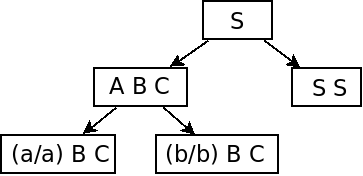
\includegraphics[width=0.5\textwidth]{search_tree.png}
  \caption{Example of a search tree}
  \label{fig:search_tree}
\end{figure}


\section{Identifying a dead end in the state tree}
A blind BFS would stop seaching a branch only when all non-terminals have been used to generate all possible end words (words with terminals only). But sometimes it is possible to tell in advance that a specific word cannot lead to the desired solution. If that is the case the whole branch can be removed from the tree. The next sections describes various ways of recognizing the dead branches.

\subsection{One of the strands is too long}
A terminal symbol which appears both in the upper or lower strand can never disappear further in the branch. That means that the count of all symbols in upper and in the lower strand must not be grater then the length of the input string. Otherwise the solution can never be reached from that branch.

\subsection{The word including non-terminals is too long}
Non-terminals present a more complex problem when dealing with the length of the word. First of all, the algorithm calculates in advance how many terminals each non-terminal produces at minimum. For instance, if the grammar contains rules: $A \rightarrow A A \:|\: \wkpair{ab}{cd} \:|\: B B$ and $B \rightarrow \wkpair{a}{\lambda}$, non-terminal $B$ produces always one terminal, that means one terminal at minimum. Non-terminal $A$ can produce various number of terminals, but two at minimum -- thanks to the rule $A \rightarrow B B$ and the fact that $B$ has the minimum of one. This value is than considered to be the length of the given non-terminal.
This length can be applied both to the upper or to the lower strand because, in general, it is not known which strand will absorb the symbols generated from the non-terminal.
This then leads to the following constraint on the word:

$$|upper| + |lower| + |nts| \geq 2 \times |input|$$

where $|upper|$ and $|lower|$ are the counts of terminals in the upper and lower strands, $|nts|$ is the length of all non-terminals in the word and $|input|$ is the length of the input string. If this constraint is broken, the word can not lead to the solution and the branch can be trimmed.


If the grammar contains no $\lambda$-rule (rule of the form $N \rightarrow ({\lambda \atop \lambda})$), This contraint guarentees that the algorithm will finish. Once all the words within the given length limit have been generated and solution not found, the search will end.

If the grammar does contain $\lambda$-rules, the previous constrain can still be applied -- the non-terminals that can be erased are assinged the length of zero. In this case, it is not possible to guarentee that the search will end, because the non-terminals of length zero can be combined infinitely many times. However, it is possible to utilize the algorithm for removing $\lambda$-rules (which is described in \cite{WK_CYK} and which is implemented in the WK\_CFG class described in the next chapter).

\subsection{The beginning of the word does not match the input}
If the current word begins with some terminal symbols in the upper strand, these symbols will always stay at the beginning further in the given branch. If these symbols do not match the prefix of the input string of the same length, the input string can never be generated from this branch.
If on the other hand, the word starts with a non-terminal, there is nothing to be said about what can be at the beginning of the word futher in the branch.

It is possible to check the end of the word in the same manner, but as it will be described futher, the generation is performed from the left to the right and so there is no benefit in checking the end.

\subsection{Checking the complementarity relation}
As previously described, the symbols in the upper and lower strands with the same indexes must be related by the complementarity relation. Unfortunately, this can be checked only at the beginning of the word. Indexes of the symbols in the middle part (anywhere after the first nonterminal) are not known. Thus this check can be understood as an extension of the previous one -- if the word begins with some terminal symbols and there are some symbols in both the upper and lower strands, these symbols can be checked if they are in the relation -- as long as its counterpart is already known.

\subsection{Checking the word correspondence to a regular expression}
It is possible to generate a regular expression that represents the current word. Each non-terminal serves as a wild card ($.*$). Each terminal in the upper strand stands for itself. Lower strand is ignored. This expression must be matchable to the input string, otherwise it is not possible to generate it from the current branch. For instance, if the word is this:
$$\wkpair{abc}{f}N_1\wkpair{d}{gh}N_2\wkpair{e}{i}N_3$$

The resulting regular expression will be: $\verb/^abc.*d.*e/$. The symbols $abc$ must be at the beginning (therefore the \verb/^/ denoting beginning of the expression); then it is not known what will be generated by the non-terminal $N_1$ -- therefore the wildcard; then there will have to be a symbol $d$; another wildcard for non-terminal $N_2$; symbol $e$; and then anything. Starting non-terminal can be represented by omitting the symbol \verb/^/ denoting the beginning of the string. Ending non-terminal can be represented by omitting the symbol \verb/$/ denoting the end of the string.

It is possible to come up with some more checks that could identify a dead end in the search tree. The disadvantage of any check is the computing power that has to be used for any node that is generated and analysed. If some checks are unlikely to significantly trim the tree and/or are complicated to compute, it is not clear if they will improve the actual performance of the algorithm.

\subsection{Examples of pruning}
Let us consider a grammar with no $\lambda$-rules with the complementarity relation being an identity, input string \verb/'abcd'/  and a following words:

\begin{enumerate}
\item{
$$\wkpair{a}{ab} N_1 \wkpair{\lambda}{cd} N_2 \wkpair{\lambda}{e}$$
The input string can never be generated from this word because the fragments of the lower strand are too long already -- it has five symbols and the input string only has four.
}
\item{
$$\wkpair{ab}{ab} N_1 N_2 \wkpair{\lambda}{d} N_3 N_4$$
This word would be promising if there had been some $\lambda$-rules. Since there are not, the word contains too many non-terminals. Each of them is going to generate at least one terminal symbol and only three symbols are missing ($c$ and $d$ in the upper strand and $c$ in the lower strand). Inevitably, there will be at least one symbol too many.
}
\item{
$$\wkpair{abd}{\lambda} N_1 \wkpair{\lambda}{ab} N_2$$
Regarless of what canb be generated from $N_1$ and $N_2$, the upper strand will always have to begin with symbols $abd$. There is no way how to insert $c$ between $b$ and $d$. Therefore the input string can never be generated from here.
}
\item{
$$\wkpair{abc}{ac} N_1 \wkpair{\lambda}{d} N_2$$
The upper strand looks promising as it starts with the same symbols $abc$ as the input string. But the lower strand starts with $ac$. The first symbol pair $(a/a)$ passes the check, the second one $(b/c)$ does not. The third symbol in the upper strand -- $c$ cannot be related to any symbol -- it has no counterpart, yet. The check was always going to end with the second symbol pair.
}
\item{
$$N_1 \wkpair{b}{\lambda} N_2 \wkpair{a}{\lambda} N_3$$
Whatever is generated from the non-terminals $N_1$, $N_2$, $N_3$ the upper strand will always keep the order of symbols -- first symbol $b$ and then symbol $a$ (with potentially some symbol before, in between and after). That can never result in the string $abcd$.
}

\section{Heuristics for node precedence} \label{heur_node_pref}

The aim of the node precedence heuristics is to choose a path in the search tree, which is likely to lead to the solution -- the more promising nodes are taken before the others and their successors are generated. The individual heuristic functions attept to answer the question -- which node is more promising than the rest? It assignes each node a number -- an evaluation of the node. The lower the node evaluation, the higher priority the node has.

Such heuristics can only be effective if the answer to the membership is positive. Unfortunately, if it is negative, it does not help that the algorithm eliminates the more promising branches of the tree first. Eventually, it will have to search through all possible states anyway in order to make sure that there is no solution.
Following node precedence heuristics have been implemented and tested.

\begin{itemize}
  \item{No heuristic -- the evaluation of the word is always 0. This is used for comparision to the other heuristics.}
  \item{Aversion to non-terminals (NTA) -- the evaluation is equal to the count of non-terminals in the word}
  \item{Weighted aversion to non-terminals (WNTA) -- each non-terminal has a precalculated weight, which is the minimum amount of rules that must be used in order to generate only terminals from it. The evaluation is equal to the sum of the weights of all non-terminals in the word.}
  \item{The terminal matching -- there are three variants that differ slightly (TM1, TM2, TM3). Each of them increases priority for each upper strand non-terminal (going from left to right), which matches the input string symbol on the same index.
  \begin{itemize}
    \item{TM1 examines terminals from the left side while ignoring non-terminals, decresing evaluation (i.e. increasing priority) for each match and finishing when it discoveres the first difference.}
    \item{TM2 is similar to TM1, but when it discovers a difference, does not finish, but increases evaluation and moves on}
    \item{TM3 evaluates the first item in the word only. If it is a non-terminal, it returns zero.}
  \end{itemize}
  }
  \item{Combinations of NTA/WNTA and TM1/TM2/TM3 -- There are six combinations, as it does not make sense to combine NTA and WNTA together.}
\end{itemize}

In summary, there are 12 node precedence heuristics considered in total (including the first, empty heuristic). Unlike in case of pruning, where all methods can be applied at the same time, there can be only one node precedence heuristic at one time. Therefore section \todo{LINK} contains the tests and comparison of the effectiveness of these heutistics.
\end{enumerate}

\section{Theoretical complexity of state space search}

\section{Parallelizing state space search algorithm}

\chapter{Implementation of the state space search} \label{chapter:implementation}

\chapter{Testing the state space search and comparison to WK-CYK}

\section{Watson-Crick grammars used for testing}

For the testing of the tree search algorithm and the WK-CYK algorithm, following Watson-Crick grammars have been used. Unless stated otherwise, the set of non-terminals and the set of terminals will simply be defined by the rules -- all the uppercase letters are non-terminals of the grammar and all the lowercase letters and digits are terminals. The starting non-terminal will be $S$ and the complementarity relation is going to be identity. With these specifications in mind the grammar can be defined by the rules only.

\begin{enumerate}
  \item{
    $$S \rightarrow \wkpair{a}{a} \:|\: S S S$$

    The accepted language is: $a(aa)^*$
  }

  \item{
    $$S \rightarrow \wkpair{a}{a} S \:|\: \wkpair{b}{b} S \:|\: \wkpair{c}{c} S \:|\: \wkpair{abc}{abc}$$

    The accepted language is: $(a+b+c)^*abc$

    The aim of this example is to test inputs with the decisive part on the very end. This could be problematic since the algorithm expands the non-terminals from left to right.
  }

  \item{
    $$S \rightarrow A \wkpair{abc}{abc}$$
    $$A \rightarrow A \wkpair{a}{a} \:|\: A \wkpair{b}{b} \:|\: A \wkpair{c}{c} \:|\: \wkpair{\lambda}{\lambda}$$

    The accepted language is: $(a+b+c)^*abc$

    The aim of this example is, again, to test inputs with the decisive part on the very end while, at the same time, the rules are left recursive.
  }

  \item{
    $$S \rightarrow Q \wkpair{a}{a} \:|\: A B C D E F G$$
    $$Q \rightarrow Q Q \:|\: A B C D E F G$$
    $$A \rightarrow \wkpair{a}{a} \:|\: \wkpair{\lambda}{\lambda}$$
    $$B \rightarrow \wkpair{b}{b} \:|\: \wkpair{\lambda}{\lambda}$$
    $$C \rightarrow \wkpair{c}{c} \:|\: \wkpair{\lambda}{\lambda}$$
    $$D \rightarrow \wkpair{d}{d} \:|\: \wkpair{\lambda}{\lambda}$$
    $$E \rightarrow \wkpair{e}{e} \:|\: \wkpair{\lambda}{\lambda}$$
    $$F \rightarrow \wkpair{f}{f} \:|\: \wkpair{\lambda}{\lambda}$$
    $$G \rightarrow \wkpair{g}{g} \:|\: \wkpair{\lambda}{\lambda}$$

    The accepted language is: $a?b?c?d?e?f?g? + (a?b?c?d?e?f?g?)^*a$ ($x?$ denotes that the symbol $x$ is optional, i.e. $(x + \epsilon)$ )

    During the transformation of this grammar to WK-CNF (more specifically, when removing the $\lambda$-rules) the number of rules increases rapidly.
  }


  \item{
    $$S \rightarrow \wkpair{a}{t} S \:|\: \wkpair{t}{a} S \:|\: \wkpair{g}{c} S \:|\: \wkpair{c}{g} A$$
    $$A \rightarrow \wkpair{c}{g} A \:|\: \wkpair{a}{t} S \:|\: \wkpair{g}{c} S \:|\: \wkpair{t}{a} B$$
    $$B \rightarrow \wkpair{c}{g} A \:|\: \wkpair{a}{t} S \:|\: \wkpair{t}{a} S \:|\: \wkpair{g}{c} C$$
    $$C \rightarrow \wkpair{a}{t} C \:|\: \wkpair{t}{a} C \:|\: \wkpair{g}{c} C \:|\: \wkpair{c}{g} C \:|\: \wkpair{\lambda}{\lambda}$$

    The complementarity relation of this grammar is: $\{(a, t), (t, a), (c, g), (g, c)\}$

    The accepted language is: $(\{a,t,c,g\}^*ctg\{a,t,c,g\}^*)^*$

    This grammar is a first step towards an actual analysis of the DNA. In this case it simply looks for the substring $ctg$
  }

  \item{
    $$S \rightarrow \wkpair{a}{\lambda} S \:|\: \wkpair{a}{\lambda} A$$
    $$A \rightarrow \wkpair{b}{a} A \:|\: \wkpair{b}{a} B$$
    $$B \rightarrow \wkpair{\lambda}{b} B \:|\: \wkpair{\lambda}{b}$$


    The accepted language is: $a^nb^n$ where $n \geq 1$
  }

  \item{
    $$S \rightarrow \wkpair{a}{a} S \wkpair{a}{a} \:|\: \wkpair{b}{b} S \wkpair{b}{b} \:|\: \wkpair{c}{c}$$

    The accepted language is: $wcw^R$ where $w \in \{a, b\}^*$($w^R$ is the reversal of string $w$)
  }

  \item{
    $$S \rightarrow \wkpair{a}{a} S \wkpair{a}{a} \:|\: \wkpair{b}{b} S \wkpair{b}{b} \:|\: \wkpair{\lambda}{\lambda}$$

    The accepted language is: $ww^R$ where $w \in \{a, b\}^*$
  }

  \item{
    $$S \rightarrow B L \:|\: R B$$
    $$L \rightarrow B L \:|\: A$$
    $$R \rightarrow R B \:|\: A$$
    $$A \rightarrow B A B \:|\: \wkpair{2}{2}$$
    $$B \rightarrow \wkpair{0}{0} \:|\: \wkpair{0}{0}$$

    The accepted language is: $x2y: x, y \in \{0,1\}^* \wedge \:|x| \neq |y|$
  }

  \item{
    $$S \rightarrow T \:|\: T \wkpair{p}{p} S$$
    $$T \rightarrow F \:|\: F T$$
    $$F \rightarrow \wkpair{e}{e} \:|\: W \:|\: \wkpair{o}{o} T \wkpair{p}{p} S \wkpair{c}{c} \:|\: X \wkpair{s}{s} \:|\: \wkpair{o}{o} Y \wkpair{c}{c} \wkpair{s}{s}$$
    $$X \rightarrow \wkpair{e}{e} \:|\: \wkpair{l}{l} \:|\: \wkpair{0}{0} \:|\: \wkpair{1}{1}$$
    $$Y \rightarrow T \wkpair{p}{p} S \:|\: F \wkpair{d}{d} T \:|\: X \wkpair{s}{s} \:|\: \wkpair{o}{o} Y \wkpair{c}{c} \wkpair{s}{s} \:|\: Z Z$$
    $$W \rightarrow \wkpair{l}{l} \:|\: Z$$
    $$Z \rightarrow \wkpair{0}{0} \:|\: \wkpair{1}{1} \:|\: Z Z$$

    The accepted language includes regular expressions over symbols 0 and 1 with parenthesis ($o$ for opening and $c$ for closing parenthesis) operators $+$ (p), $*$ (s), $\cdot$ (d) and symbols $\emptyset$ (e), $\varepsilon$ (l)
  }

  \item{
    $$S \rightarrow A \:|\: B \:|\: A B \:|\: B A$$
    $$A \rightarrow \wkpair{a}{a} \:|\: \wkpair{a}{a} A \wkpair{a}{a} \:|\: \wkpair{a}{a} A \wkpair{b}{b} \:|\: \wkpair{b}{b} A \wkpair{b}{b} \:|\: \wkpair{b}{b} A \wkpair{a}{a}$$
    $$B \rightarrow \wkpair{b}{b} \:|\: \wkpair{a}{a} B \wkpair{a}{a} \:|\: \wkpair{a}{a} B \wkpair{b}{b} \:|\: \wkpair{b}{b} B \wkpair{b}{b} \:|\: \wkpair{b}{b} B \wkpair{a}{a}$$

    The accepted language is: $\{a, b\}^* \setminus ww$ where $w \in \{a, b\}^*$ -- i.e. the complement of the copy language.
  }

  \item{
    $$S \rightarrow \wkpair{r}{\lambda} S \:|\: \wkpair{r}{\lambda} A$$
    $$A \rightarrow \wkpair{d}{r} A \:|\: \wkpair{d}{r} B$$
    $$B \rightarrow \wkpair{u}{d} B \:|\: \wkpair{u}{d} C$$
    $$C \rightarrow \wkpair{r}{u} C \:|\: \wkpair{r}{u} D$$
    $$D \rightarrow \wkpair{\lambda}{r} D \:|\: \wkpair{\lambda}{r}$$

    The accepted language is: $r^nd^nu^nr^n$ where $n \geq 1$
  }

  \item{
    $$S \rightarrow \wkpair{a}{\lambda} S \wkpair{b}{\lambda} \:|\: \wkpair{a}{\lambda} A \wkpair{b}{\lambda}$$
    $$A \rightarrow \wkpair{c}{a} A \:|\: \wkpair{\lambda}{c} B \wkpair{\lambda}{b}$$
    $$B \rightarrow \wkpair{\lambda}{c} B \wkpair{\lambda}{b} \:|\: \wkpair{\lambda}{\lambda}$$

    The accepted language is: $a^nc^nb^n$ where $n \geq 1$
  }

  \item{
    $$S \rightarrow \wkpair{a}{\lambda} S \:|\: \wkpair{a}{\lambda} A$$
    $$A \rightarrow \wkpair{b}{\lambda} A \:|\: \wkpair{b}{\lambda} B$$
    $$B \rightarrow \wkpair{c}{a} B \:|\: \wkpair{c}{a} C$$
    $$C \rightarrow \wkpair{d}{b} C \:|\: \wkpair{d}{b} D$$
    $$D \rightarrow \wkpair{\lambda}{c} D \:|\: \wkpair{\lambda}{d} D \:|\: \wkpair{\lambda}{\lambda}$$

    The accepted language is: $a^nb^mc^nd^m$ where $n, m \geq 1$
  }

  \item{
    $$S \rightarrow \wkpair{a}{\lambda} S \:|\: \wkpair{b}{\lambda} S \:|\: \wkpair{c}{\lambda} A$$
    $$A \rightarrow \wkpair{a}{a} A \:|\: \wkpair{b}{b} A \:|\: \wkpair{\lambda}{c} B$$
    $$B \rightarrow \wkpair{\lambda}{a} B \:|\: \wkpair{\lambda}{b} B \:|\: \wkpair{\lambda}{\lambda}$$

    The accepted language is: $wcw$ where $w \in \{a, b\}^*$
  }

  \item{
    $$S \rightarrow \wkpair{a}{\lambda} S \wkpair{a}{a} \:|\: \wkpair{a}{\lambda} A \wkpair{a}{a} $$
    $$A \rightarrow \wkpair{bb}{a} A \:|\: \wkpair{bbb}{a} A \:|\: \wkpair{\lambda}{b} B$$
    $$B \rightarrow \wkpair{\lambda}{b} B \:|\: \wkpair{\lambda}{\lambda}$$

    The accepted language is: $a^nb^ma^n$ where $2n \leq m \leq 3n$
  }

  \item{
    $$S \rightarrow S S \:|\: \wkpair{a}{a} S \wkpair{b}{b} \:|\: \wkpair{a}{\lambda} S \:|\: \wkpair{a}{\lambda} A$$
    $$A \rightarrow \wkpair{b}{a} A \:|\: \wkpair{b}{a} B \:|\: \wkpair{b}{a}$$
    $$B \rightarrow \wkpair{\lambda}{b} B \:|\: \wkpair{\lambda}{b} \:|\: B B \:|\: \wkpair{a}{a} S \wkpair{b}{b} \:|\: \wkpair{a}{\lambda} S \:|\: \wkpair{a}{\lambda} A$$

    The accepted language is: $w: \#_a(w) = \#_b(w)$ and for any prefix $v$ of $w: \#_a(v) \geq \#_b(v)$  where $\#_a(x)$ denotes the number of occurrences of symbol $a$ in string $x$
  }

  \item{
    $$S \rightarrow \wkpair{l}{\lambda} S \:|\: \wkpair{l}{\lambda} A$$
    $$A \rightarrow \wkpair{r}{l} A \:|\: \wkpair{r}{l} B$$
    $$B \rightarrow \wkpair{l}{r} B \:|\: \wkpair{\lambda}{r} B \:|\: \wkpair{\lambda}{\lambda} \:|\: A$$

    The accepted language is: $(l^n r^n)^k$ where $n$ does not increase for subsequent $k$. For instance: $lllrrrlrlr$ is within the language, $llrrlllrrr$ is not.
  }

  \item{
    The grammar is identical to the grammar 13 with a difference in the complementarity relation. Relations between symbols $a, b$ and symbols $a, c$ are added.

    This means that the relation is: $\rho = \{(a, a), (b, b), (c, c), (a, b), (b, a), (a, c), (c, a)\}$

    The accepted language is: $a^n b^m c^n$ where $n, m \geq 1$
  }

  \item{
	The grammar is identical to the grammar 14 with a difference in the complementarity relation. Relation between symbols $a, b$ is added making the relation $\rho = \{(a, a), (b, b), (c, c), (d, d), (a, b), (b, a)\}$

	The accepted language is: $a^m b^n c^o d^p$ where $m, n, o, p \geq 1 \wedge m+n = o+p$
  }


\end{enumerate}

There are twenty grammars altogether. Grammars 1--5 are regular, 6--11 are context-free and 12--18 are context-sensitive. Grammars 19 and 20 are context-free but they also have a non-bijective complementarity relation.

In reality, there are not 20 but 40 grammars, because all of them are going to be used in the basic form and after the transformation to the Chomsky normal form. That results in a different grammar (although accepting the same language) which is usually significantly more difficult to calculate with, as there are more rules and many rules generate more non-terminals.

\section{Testing the state space search}

There is a lot of parameters that could be tested and analysed. How efficient are the various heuristics (both pruning and node preference) for different grammars. What inputs lengths are answered withing a reasonable time frame? Or more generally -- what is the relation between input length and time to get the answer? What are the memory requirements? What is the difference in decition time between input strings which are in the given language and those which are not? Is there a difference between some inputs of the same lengths?

In order to analyse these questions, I have decided to test the state space search in the following stages.
\begin{enumerate}
  \item{Comparison of the node precedence heuristics and analysis of their efficiency.}
  \item{Comparison of the pruning heuristics and analysis of their efficiency.}
  \item{Analysis of the time and memory complexity based on the length of the input string for all grammars.}
  \item{Testing if there are any different inputs of the same length which would result in a significant difference in the computation complexity.}
  \item{Testing the WK-CYK algorithm with various grammars and inputs and comparision to the state space search.}
\end{enumerate}

\subsection{Comparison of the node precedence heuristics efficiency}
In section \ref{heur_node_pref}, 12 node precedence heuristics have been described and only one of them can be active at a time.

The space state search algorithm contains five different tests of pruning the state tree (which can and usually do work at the same time) and five rule precedence heuristics (of which only one is active). In order to compare their effectiveness I used the script \textit{node\_prec\_heuristic\_compare.py} which runs one test for each of the 40 grammars with an input that will be accepted. It is not useful to test node precedence heuristics with inputs that are not withing the given language as in such cases, the whole space state needs to be searched and node precedence cannot help in any way. The input strings have been chosen to have suitable lengths, so that the computation is finished (at least with some heuristics) in a reasonable time -- specifically within the time limit of ten seconds, but also to last some measurable amount of time.

Each of the 40 tests is run 12 times with a different node precedence heuristic. There are three metrics to observe:
\begin{itemize}
  \item{How many times the search timeouted?}
  \item{What the total time in which all 40 tests were completed is for each heuristic. There should be a kind of penalty involved if the test timeouts, because the time needed for the computation is in that case certainly greater then the time it actually ran, before it got stopped by the time limit. Therefore for the sake of the comparison, the time need is in this case doubled.}
  \item{The total time normalized for each test -- the time of the fastest heuristic for each test is normalized to one. This is probably the most telling metric as each test has roughly the same impact on the final number.}
\end{itemize}

Each test prints out the results in a table similar to \ref{tab:node_heuristics_table}. The upper part of the table displays the description of the accepted language, number of rules, non-terminals and terminals, string on the input, whether the input is expected to be accepted and time limit. In the lower part the table shows for each of the node precedence heuristic how much time it took, how many states were in the queue and how many were analysed, how many times each pruning heuristic was used (SL -- strands too long, TL -- strands is too long including the non-terminals, WS -- word does not match the input, RL -- complementarity relation failed, RE -- regular expression check failed) and the result of the search (True, False or Timeout). It would not be practical to present here the complete output, but it can be recreated simply by running the script again and is also attached in the file \textit{output/node\_prec\_heuristic.txt}.

\begin{figure}[h]
  \caption{An output of the node precedence heuristics test}
  \label{tab:node_heuristics_table}
\begin{tabular}{ |l|l|l|l|l|  }
  \hline
  \multicolumn{5}{|l|}{Test 1} \\
  \hline
  Grammar & \multicolumn{4}{|l|}{$a(aa)^*$} \\
  Rules / NTs / Ts & \multicolumn{4}{|l|}{2/1/1} \\
  Input string & \multicolumn{4}{|l|}{aaaaaaaaaaaaaaaaaaaaaaaaa... [len 801]} \\
  Should accept & \multicolumn{4}{|l|}{Yes} \\
  Timeout & \multicolumn{4}{|l|}{7 seconds} \\
  \hline
  Strategy & Time & States Q+C & Prunes (SL, TL, WS, RL, RE)& Accepted \\
  \hline
 NTA & 0.4886 & 994 + 3001  & 0, 5, 0, 0, 250 & TRUE \\
 WNTA & 0.4189 & 498 + 2503 & 0, 3, 0, 0, 250 & TRUE  \\
 TM1 & 0.739 & 1489 + 3994 & 0, 7, 0, 0, 249  & TRUE  \\
 TM2 & 0.7385 & 1489 + 3994 & 0, 7, 0, 0, 249 & TRUE  \\
 TM3 & 0.7366 & 1489 + 3994 & 0, 7, 0, 0, 249  & TRUE  \\
 NTA+TM1 & 0.5903 & 992 + 2999 & 0, 5, 0, 0, 250 & TRUE  \\
 NTA+TM2 & 0.5915 & 992 + 2999 & 0, 5, 0, 0, 250 & TRUE  \\
 NTA+TM3 & 0.5923 & 992 + 2999 & 0, 5, 0, 0, 250 & TRUE  \\
 WNTA+TM1 & 0.495 & 498 + 2503 & 0, 3, 0, 0, 250 & TRUE  \\
 WNTA+TM2 & 0.4949 & 498 + 2503 & 0, 3, 0, 0, 250 & TRUE  \\
 WNTA+TM3 & 0.4977 & 498 + 2503 & 0, 3, 0, 0, 250 & TRUE  \\
 no heuristic & 2.4445 & 4188 + 22147 & 0, 89, 0, 0, 239 & TRUE  \\
  \hline
  \hline
\end{tabular}
\end{figure}

It is interensting to note that different heuristics are better in different test cases. This is illustrated by selected test cases which are on figure \ref{fig:selected_tests}. There are some case when the best heuristic is the empty one, which assigned zero to each node, like in case of test 23. This is because this heuristic is the simpliest to compute and if no heuristic is effective in a particular test case, this one wins. But it does not win by a large margin, so these cases are not decisive.

In some cases, a certain heuristics don't work so well, but their combination does. This can be seen in test 22 -- NTA and WNTA have poor result, comparable to no heuristic. TM1, TM2, TM3 have somewhat better result, but by far the best result is achieved by combination of NTA with any version of TN.

\begin{figure}[h]
  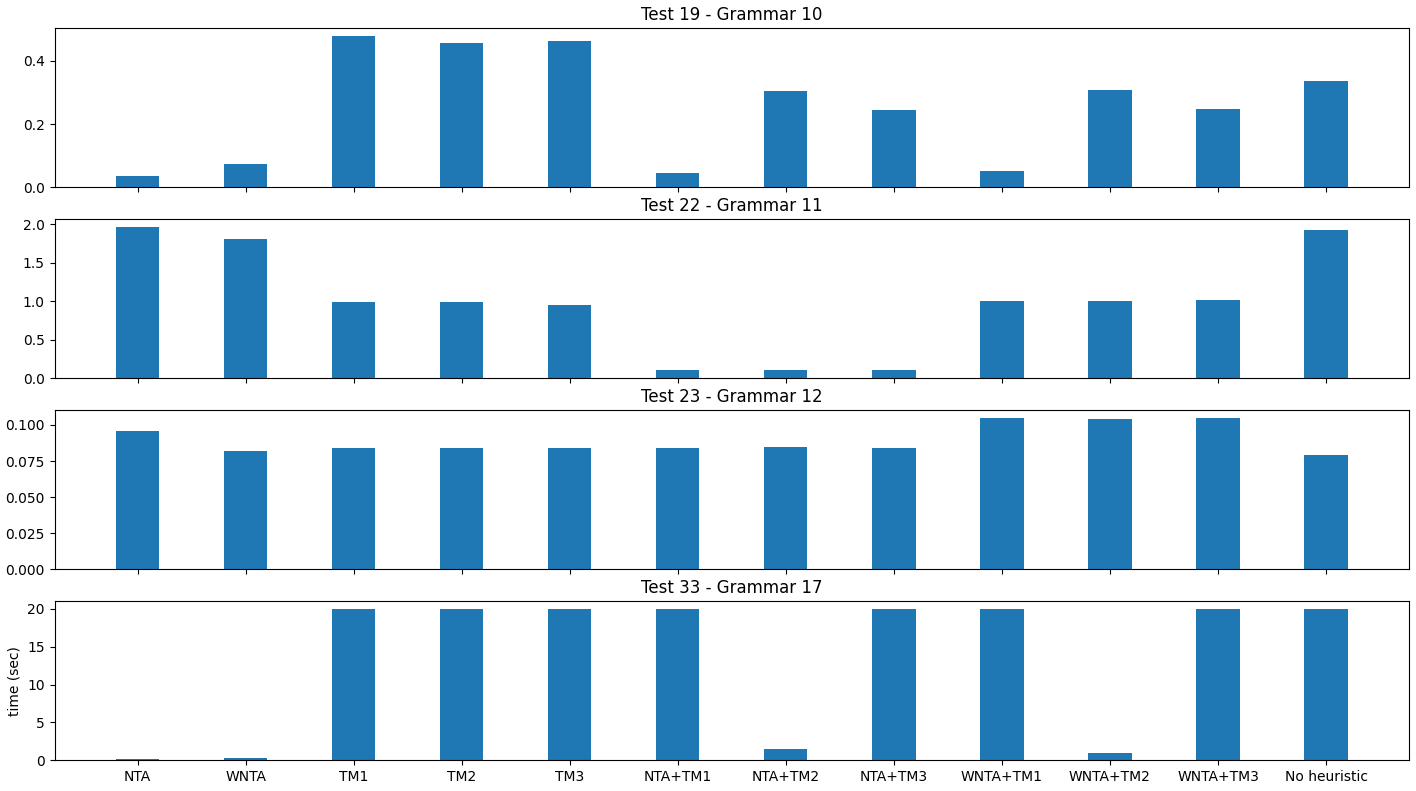
\includegraphics[scale=0.42]{four_heur_tests.png}
  \caption{Selected comparisons of node precedence heuriscits}
  \label{fig:selected_tests}
\end{figure}

The figure \ref{fig:node_heuristics_comp} shows the total result for all of the 40 tests. It is clear that the best results are achieved by the combination NTA, TM2. This heuristic did not timeout in any of the tests and overall is the fastest. Even if in some cases there are some faster heuristics, it's usually not by much.

\begin{figure}[h]
  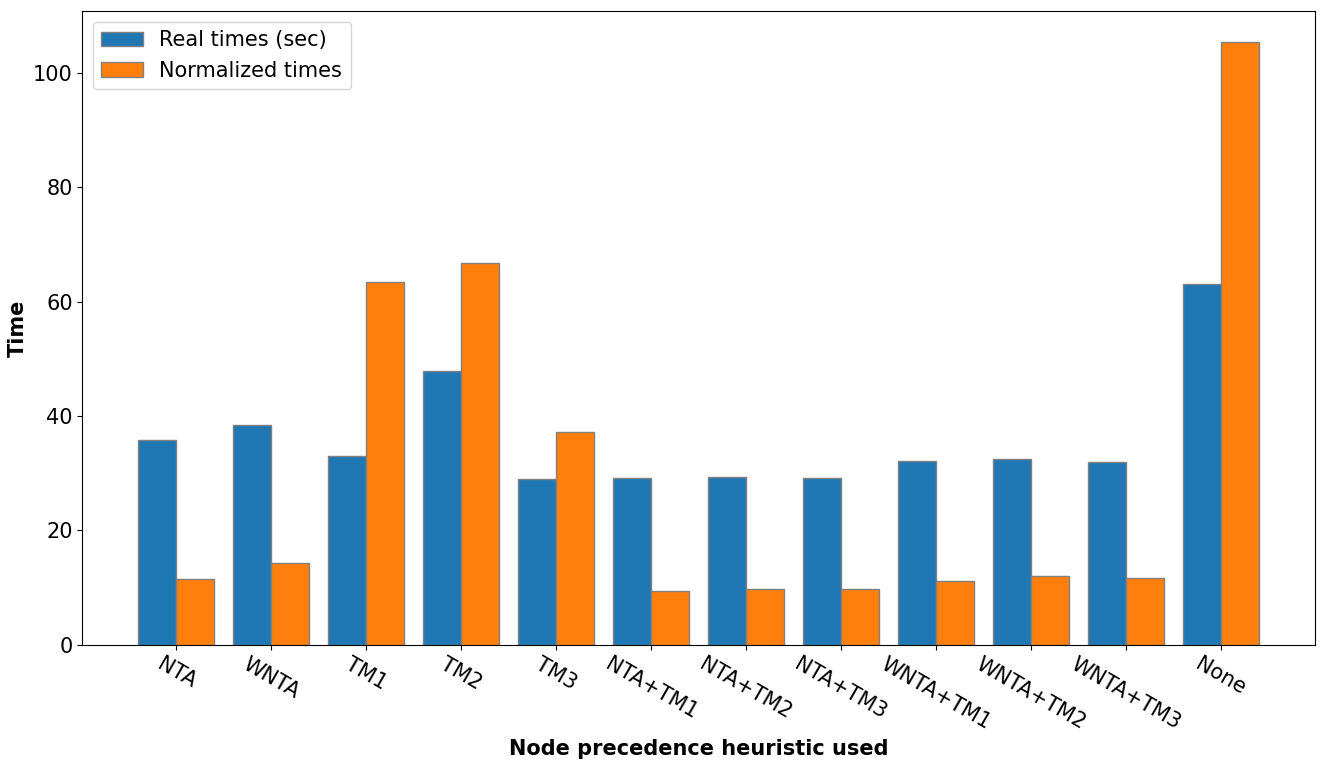
\includegraphics[scale=0.44]{node_heuristics_comp.png}
  \caption{Comparison of the node precedence heuristic functions}
  \label{fig:node_heuristics_comp}
\end{figure}

\subsection{Comparison of the pruning heuristics efficiency}

Pruning has the advantage of being useful whether the input string is going to be accepted or rejected by the tree search. Also, all of the pruning can be on at the same time -- each node can be checked by all available check to see if it can be pruned or not.

The testing is performed over 80 tests -- each of the 40 grammars is used for a positive test (where the input will be accepted) and a negative test (input will be rejected).
Each test contains seven runs of the tree search algorithm -- one where all pruning heuristics are on, one where all are turned off, and one for each heuristic where all are turned on except the given one.

Similarly to the node precedence heuristics comparison, the metrics that are important are the total time needed to compute the 80 tests and a number of timeouts.

The tests can be run by the script \textit{pruning\_heuristic\_compare.py} and each test print out a table similar to the table \ref{tab:prune_heuristics_table}. Again, it would not be practical to include the entire output here. The complete set of results can be recreated by running the script again and it is included in file \textit{output/prune\_heuristic.txt}.

\begin{figure}[h]
  \caption{An output of the pruning heuristics test}
  \label{tab:prune_heuristics_table}
\begin{tabular}{ |l|l|l|l|l|  }
  \hline
  \multicolumn{5}{|l|}{Test 1} \\
  \hline
  Grammar & \multicolumn{4}{|l|}{$a(aa)^*$} \\
  Rules / NTs / Ts & \multicolumn{4}{|l|}{2/1/1} \\
  Input string & \multicolumn{4}{|l|}{aaaaaaaaaaaaaaaaaaaaaaaaa... [len 801]} \\
  Should accept & \multicolumn{4}{|l|}{Yes} \\
  Timeout & \multicolumn{4}{|l|}{7 seconds} \\
  \hline
  Strategy & Time & States Q+C & Prunes (SL, TL, WS, RL, RE)& Accepted \\
  \hline
  ALL ON & 0.7841 & 799 + 1200 & 0, 3, 0, 0, 400 & TRUE \\
  strands len OFF & 0.7781 & 799 + 1200 & 0, 3, 0, 0, 400 & TRUE \\
  total len OFF & 0.7799 & 801 + 1200 & 0, 0, 0, 0, 400 & TRUE \\
  terms match OFF & 0.7705 & 799 + 1200 & 0, 3, 0, 0, 400 & TRUE \\
  relation OFF & 0.655 & 799 + 1200 & 0, 3, 0, 0, 400 & TRUE \\
  regex OFF & 0.3594 & 800 + 1599 & 0, 3, 0, 0, 0 & TRUE \\
  ALL OFF & 0.2179 & 801 + 1600 & 0, 0, 0, 0, 0 & TRUE \\
  \hline
  \hline
\end{tabular}
\end{figure}

The summary is displayed on Figures \ref{fig:prune_timeouts_comp} -- the number of timeouts and \ref{fig:prune_times_comp} -- the amount of time for each of the seven cases across the 80 tests. The smaller the individual bars are, the better the result. But in case of the bars representing a specific pruning heuristic being turned off, the bigger the bar, the more important the given heuristic is, because the result is that much worse without it.

\begin{figure}[h]
  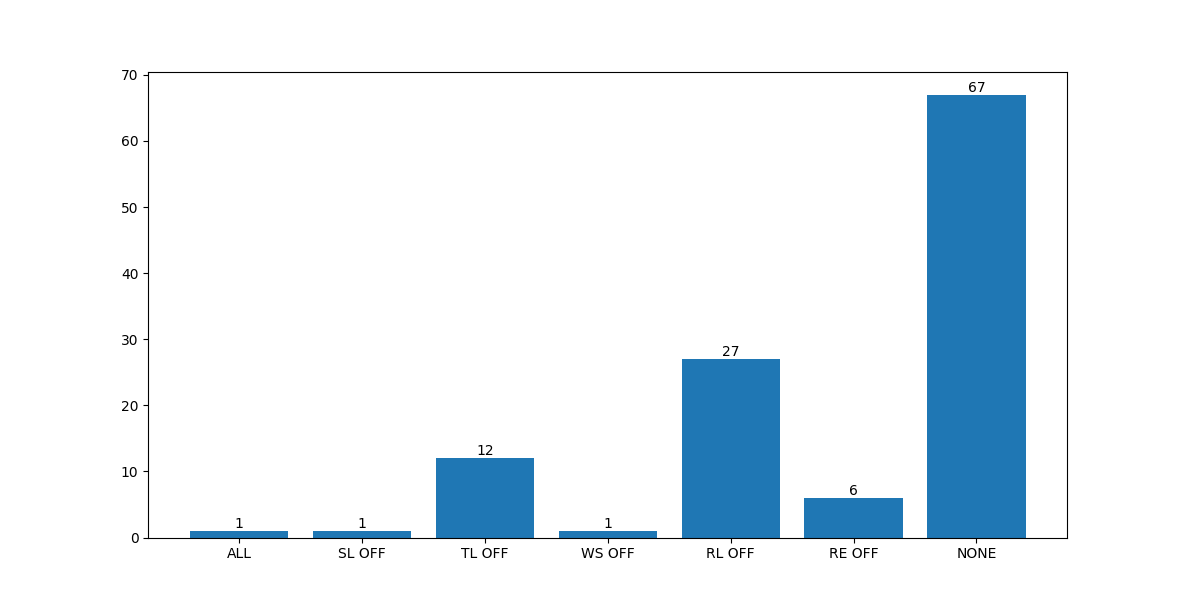
\includegraphics[scale=0.5]{prune_timeouts_comp.png}
  \caption{TIMEOUTS}
  \label{fig:prune_timeouts_comp}
\end{figure}

\begin{figure}[h]
  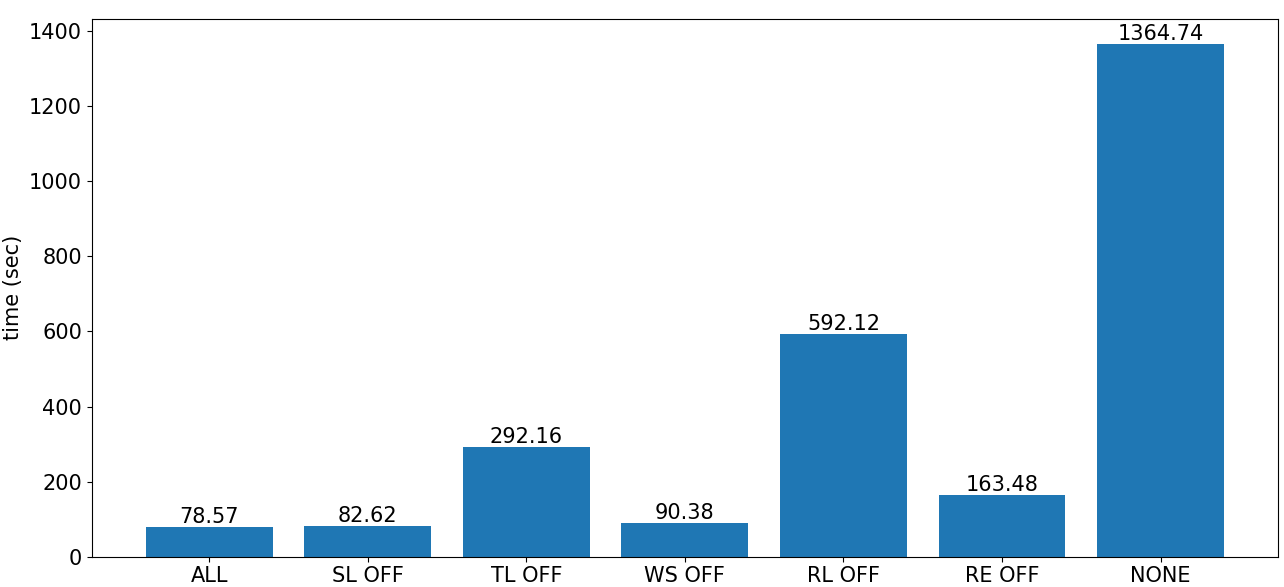
\includegraphics[scale=0.7]{prune_times_comp.png}
  \caption{TOTAL TIMES}
  \label{fig:prune_times_comp}
\end{figure}


From these results it is clear that the tree pruning is the key feature of the tree search algorithm. After turning off the pruning, the results are very poor -- 67 out of 80 tests timeouted. The total time is then not relvant at all. The middle bars representing the individual pruning heuristics turned off needs to be compared to the first one, where all heuristics are on, to see how important the given heuristic actually is. Thus the figure suggests, that the RL (complementarity relation) check si the most important one, because turning it off had the biggests impact on the result. This can be a bit misleading, as some heuristics can be sometimes backed up by another one. This is the reason why the WS (match of leftmost terminals and the input string) seem to have a rather small impact. If this heuristic is turned off, the dead branch can be idntified by the RE (regular expression) check and so the impact is not so big. Similarly, turning off the SL (strands length) heuristic is of smaller impact, because it is backed up by TL (total length) heuristic.

Nevertheless, all heuristic are useful according to this result, because no other bar is as small as the first one. This means that the best result is achieved when all heuristics are on at the same time. This is especially important in the case of the RE heuristic. This one is quite demanding with regards to computation power -- regular expression match is performed each time this check is executed. Therefore it is the last check that is used, if there is another heuristic able to prune the node, a lot of computational power is saved. However, the figure shows clearly, that the RE heuristic contributes significantly to the overall performance (still, some tests cannot take advantage of this heuristic and turning it off would improve the results).



\subsection{Analysis of the memory requirements}
The tree search algorithm needs to keep in memory the nodes, which have been generated but not yet analyzed. These are the states in the queue. Also, it keeps track of all nodes which have already been generated. Those are the states that had been in the queue before and states that are there at the moment, as in both cases, there is no reason to put them into the queue again. There is no need to keep in memory the states that have been generated, their hash is enough.

Then it is necessary to remember states in the queue, the number of the states there can go up or down as the search progresses, but it is more likely to go up, unless the search is coming to an end. In any case, the important figure is the maximum number of states, that were in the queue at one point.

Next parameter that needs to be considered is the size of one state in the memory. As mentioned in the section \ref{chapter:implementation}, there are six integers (storing the number of terminals in the two strands, number of nonterminals, hash number, the node parent and the node precedence evaluation) and the word itself. The word can contain up to twice the number of symbols then is the length of the input string. If it contains more, it is going to be pruned.

This is not necessarily true, if the grammar contains some $\lambda$-rules and non-terminals that can be erased. Then the theoretical length of the word in memory has no limit, but this is not a typical scenario and can be avoided altogether by applying the $\lambda$-rules removal algorithm.

The equation for getting the memory requirement based on the number of states working with is than the following:

$$S_{all} \times size(int) + S_{open} \times (6 \times size(int) + 2 \times size(symbol) \times |input|)$$

$S_{all}$ is the number of all states generated, $S_{open}$ is the maximum number of states in the queue, $size(int)$ is the size of an integer (for this calculation, I will assume it is 64 bytes), $size(symbol)$ is the size of one symbol of the grammar and $|input|$ is the length of the input string.

However, current implementation has more memory consumption. This is because when an input is accepted, it may be interesting to know what path from the starting non-terminal to the goal has been discovered. In order to do that, the program needs to retain all the states that have been analysed, storing their hashes is not enough.

I've chosen grammar 3 in CNF to test the results in practise, as this grammar is among the hardest ones with respect to computing complexity. I used inputs in the form of $a^nb$ with increasing $n$, which will always be rejected, beacuse the grammar accepts strings that end with $abc$.

The figure \ref{fig:mem_consumption} on the left show the amount of memory requirements in relation to the input length and in the middle in relation to the time needed. To the right is the experimental result where I measured real memory comsuption of the program in time.

\begin{figure}[h]
  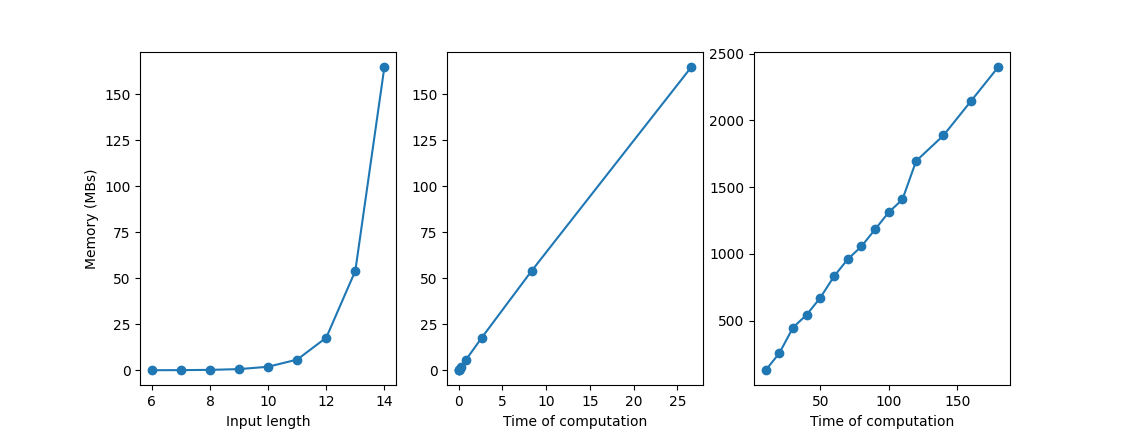
\includegraphics[scale=0.5]{mem_consumption.png}
  \caption{Memory consumption of tree search}
  \label{fig:mem_consumption}
\end{figure}



\subsection{The time complexity of the state space search}
The previous sections showed, that the best overall performance is achieved when using all of the tree pruning heuristics and using the NTA+TM2 as the node precedence heuristic. This may not be the case for every grammar or every input, but it is the case most of the time. Therefore this will be the setting used in following sections --- for testing the tree search performance, analysing the practical complexity and comparing to WK-CYK algorithm.

I used script \textit{input\_compl\_compare.py} to test the time complexity in relation to the input length. It runs 80 test, two for each of the 40 grammars --- one with inputs that are in the language defined by the grammar and so the inputs are going to be accepted --- and one with inputs which will be refused. Each test runs the tree search several times and increases the input length. It stops when the computation takes longer than a limit of ten seconds or after 30 runs. For each of the 80 tests it prints out table similar to \ref{tab:input_compl_test}. As it would not be practical to present all of the results here, they cen be recreated by simply running the script again and they are included in the file \textit{output/input\_complexity\_test.txt}.

\begin{figure}[h]
  \caption{An output of the time complexity test}
  \label{tab:input_compl_test}
\begin{tabular}{ |l|l|l|l|l|  }
  \hline
  \multicolumn{5}{|l|}{Test 1} \\
  \hline
  Grammar & \multicolumn{4}{|l|}{$a(aa)^*$} \\
  Rules / NTs / Ts & \multicolumn{4}{|l|}{2/1/1} \\
  Should accept & \multicolumn{4}{|l|}{Yes} \\
  Timeout & \multicolumn{4}{|l|}{7 seconds} \\
  \hline
  Input length & Time & States Q+C & Prunes (SL, TL, WS, RL, RE)& Accepted \\
  \hline
 501 & 0.3362 & 499 + 750 & 0, 3, 0, 0, 250 & TRUE \\
 601 & 0.4482 & 599 + 900 & 0, 3, 0, 0, 300 & TRUE \\
 701 & 0.5978 & 699 + 1050 & 0, 3, 0, 0, 350 & TRUE \\
 801 & 0.7744 & 799 + 1200 & 0, 3, 0, 0, 400 & TRUE \\
 901 & 0.9728 & 899 + 1350 & 0, 3, 0, 0, 450 & TRUE \\
 1001 & 1.1931 & 999 + 1500 & 0, 3, 0, 0, 500 & TRUE \\
 1101 & 1.4367 & 1099 + 1650 & 0, 3, 0, 0, 550 & TRUE \\
 1201 & 1.6959 & 1199 + 1800 & 0, 3, 0, 0, 600 & TRUE \\
 1301 & 1.9928 & 1299 + 1950 & 0, 3, 0, 0, 650 & TRUE \\
 1401 & 2.3087 & 1399 + 2100 & 0, 3, 0, 0, 700 & TRUE \\
 1501 & 2.6799 & 1499 + 2250 & 0, 3, 0, 0, 750 & TRUE \\
 1601 & 3.0023 & 1599 + 2400 & 0, 3, 0, 0, 800 & TRUE \\
 1701 & 3.3801 & 1699 + 2550 & 0, 3, 0, 0, 850 & TRUE \\
 1801 & 3.776 & 1799 + 2700 & 0, 3, 0, 0, 900 & TRUE \\
 1901 & 4.2107 & 1899 + 2850 & 0, 3, 0, 0, 950 & TRUE \\
 2001 & 4.6528 & 1999 + 3000 & 0, 3, 0, 0, 1000 & TRUE \\
 2101 & 5.1277 & 2099 + 3150 & 0, 3, 0, 0, 1050 & TRUE \\
 2201 & 5.6251 &2199 + 3300 & 0, 3, 0, 0, 1100 & TRUE \\
 2301 & 6.134 & 2299 + 3450 & 0, 3, 0, 0, 1150 & TRUE \\
 2401 & 6.665 & 2399 + 3600 & 0, 3, 0, 0, 1200 & TRUE \\
 2501 & 7.3398 & 2499 + 3750 & 0, 3, 0, 0, 1250 & TRUE \\
 2601 & 8.057 & 2599 + 3900 & 0, 3, 0, 0, 1300 & TRUE \\
 2701 & 8.4195 & 2699 + 4050 & 0, 3, 0, 0, 1350 & TRUE \\
 2801 & 9.2167 & 2799 + 4200 & 0, 3, 0, 0, 1400 & TRUE \\
 2901 & 10.3625 & 2899 + 4350 & 0, 3, 0, 0, 1450 & TRUE \\
  \hline
  \hline
\end{tabular}
\end{figure}

Different grammars have very different complexity as the following results show. The following graphs display result for each of the 20 grammars.

% Figure \ref{fig:res_grammar_1} shows results for grammar 1. 

\begin{figure}[h]
  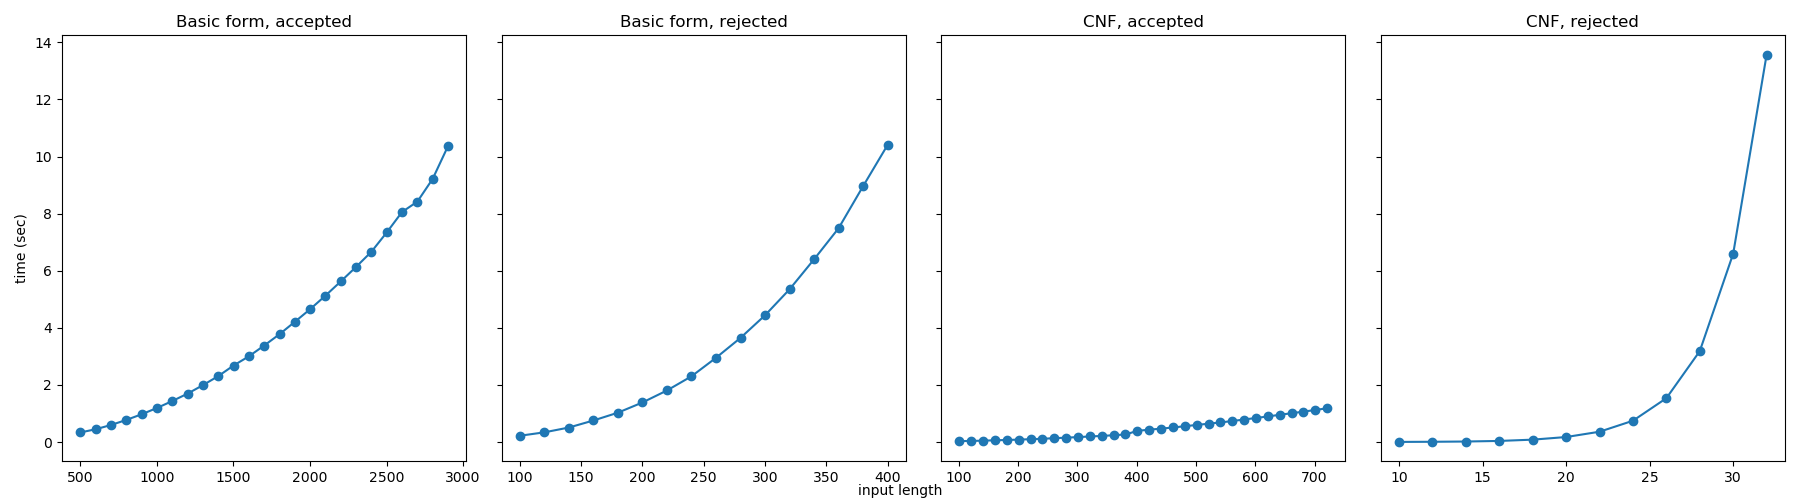
\includegraphics[scale=0.33]{compl_result_grammar_1.png}
  \caption{Grammar 1: $a(aa)^*$}
  \label{compl_result_grammar_1}
\end{figure}

\begin{figure}[h]
  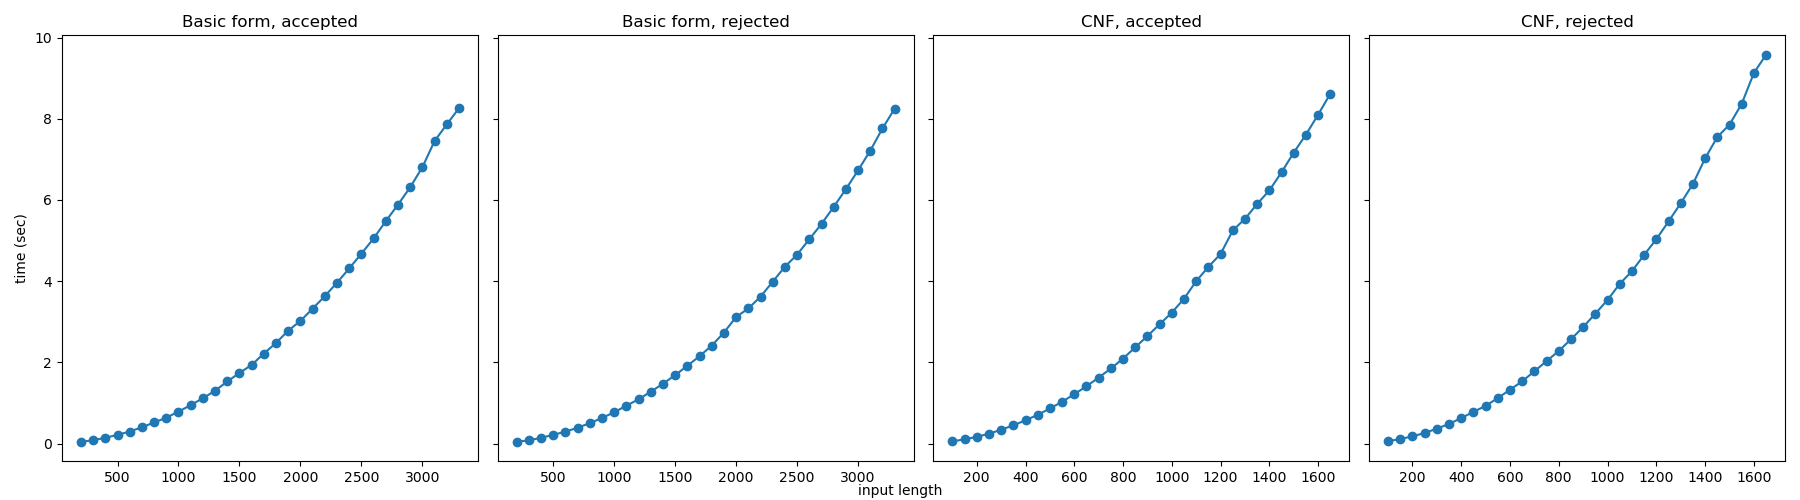
\includegraphics[scale=0.33]{compl_result_grammar_2.png}
  \caption{Grammar 2: $(a+b+c)^*abc$ left recursive rules}
  \label{compl_result_grammar_2}
\end{figure}

\begin{figure}[h]
  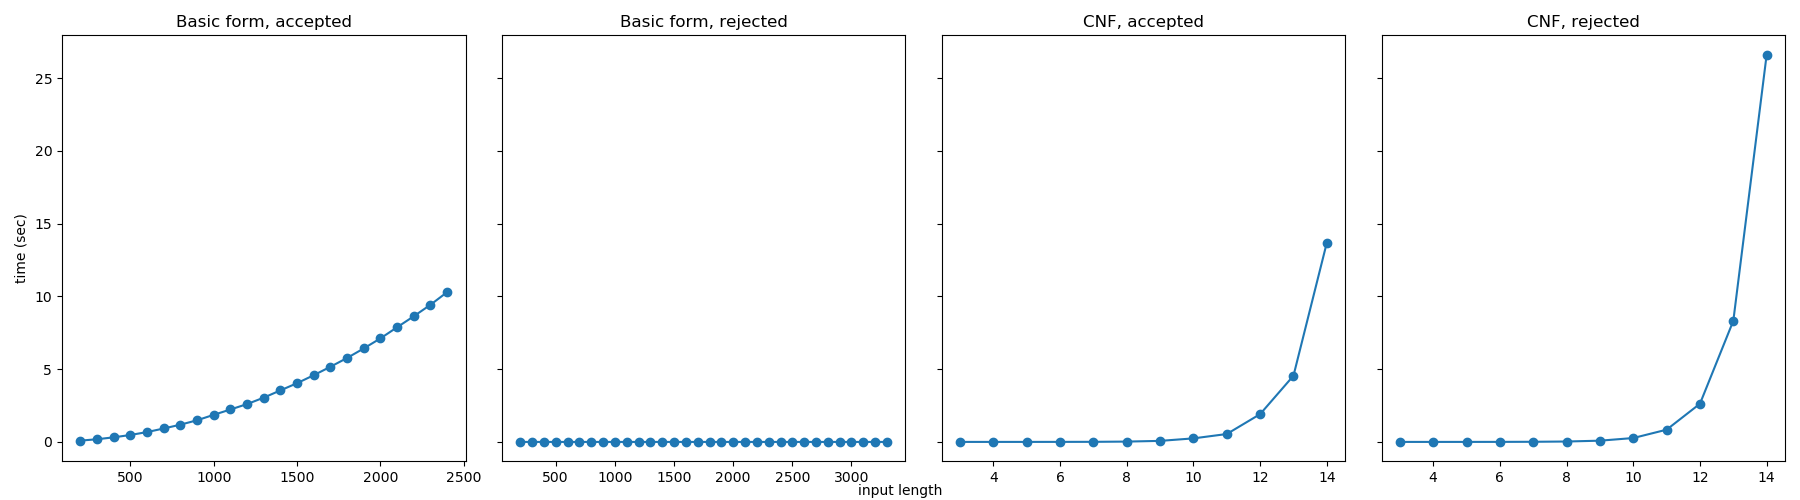
\includegraphics[scale=0.33]{compl_result_grammar_3.png}
  \caption{Grammar 3: $(a+b+c)^*abc$ right recursive rules}
  \label{compl_result_grammar_3}
\end{figure}

\begin{figure}[h]
  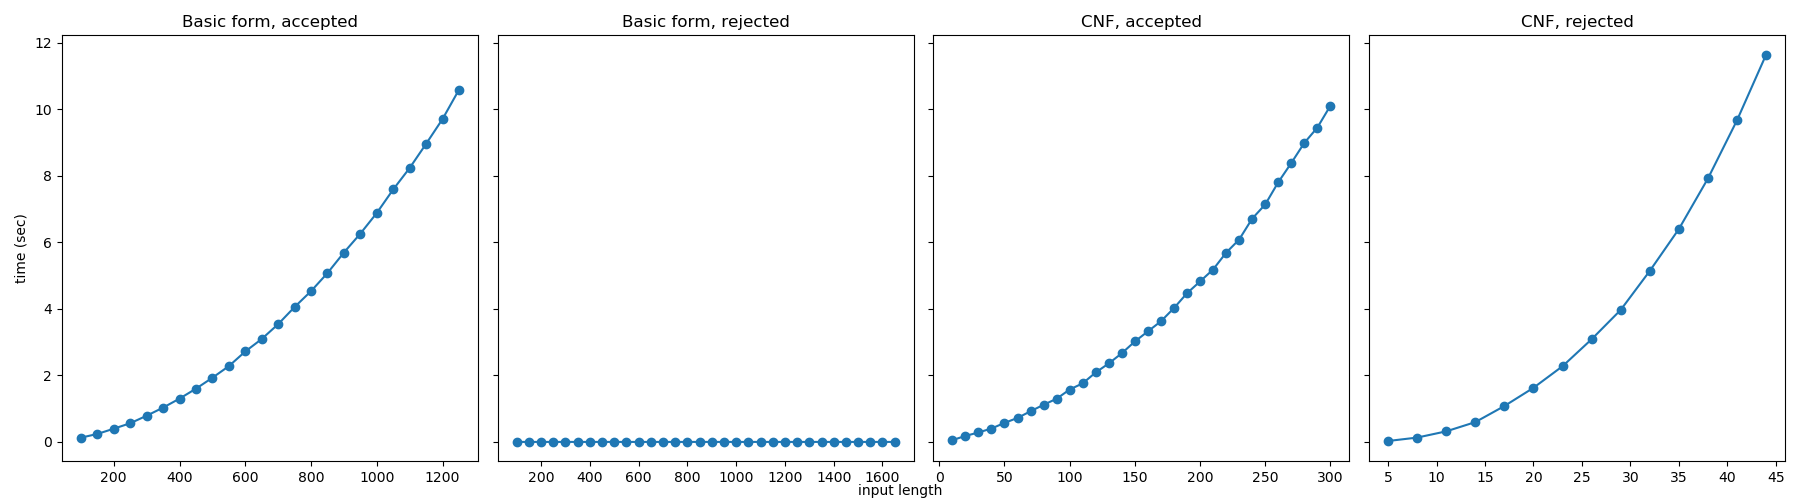
\includegraphics[scale=0.33]{compl_result_grammar_4.png}
  \caption{Grammar 4: $a?b?c?d?e?f?g? + (a?b?c?d?e?f?g?)^*a$}
  \label{compl_result_grammar_4}
\end{figure}

\begin{figure}[h]
  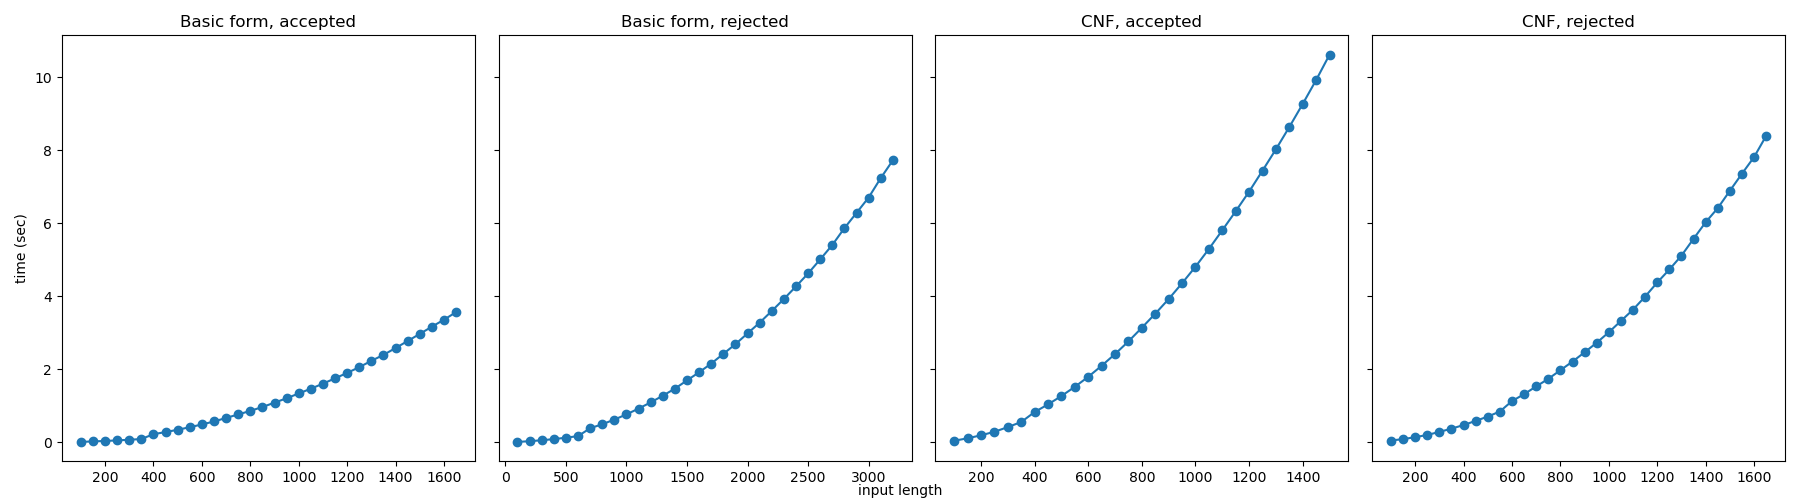
\includegraphics[scale=0.33]{compl_result_grammar_5.png}
  \caption{Grammar 5: $(\{a,t,c,g\}^*ctg\{a,t,c,g\}^*)^*$}
  \label{compl_result_grammar_5}
\end{figure}

\begin{figure}[h]
  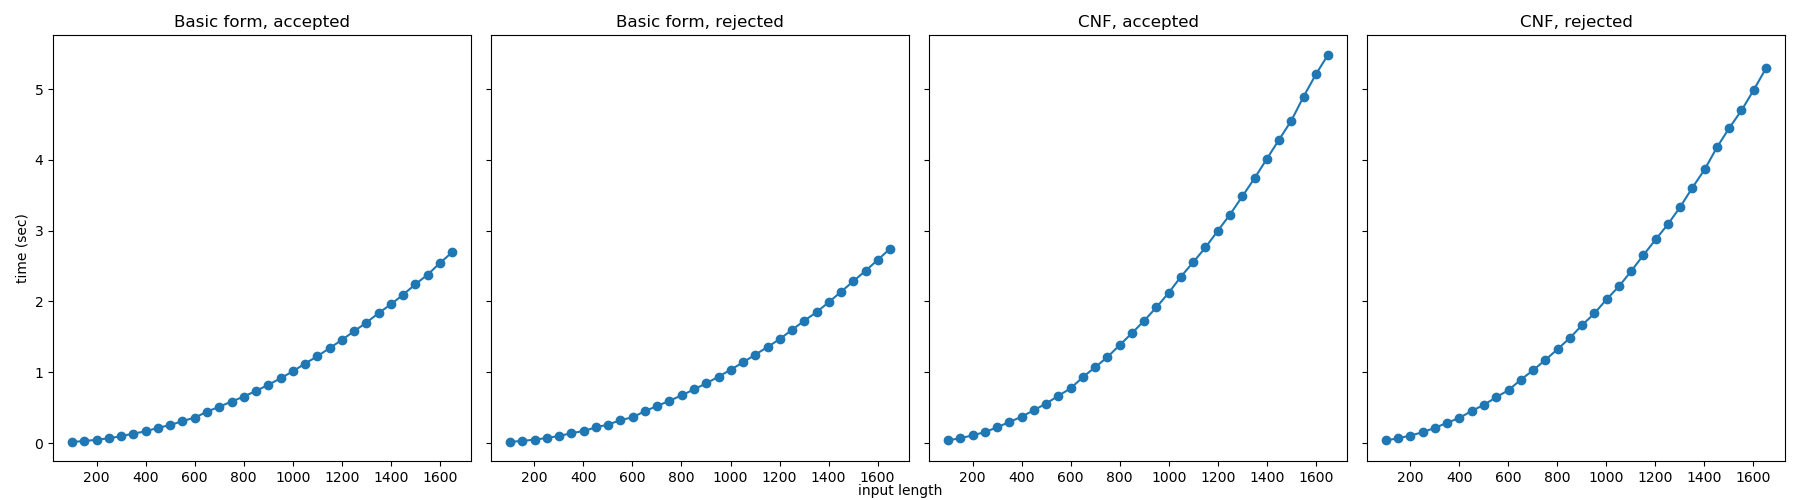
\includegraphics[scale=0.33]{compl_result_grammar_6.png}
  \caption{Grammar 6: $a^n b^n$}
  \label{compl_result_grammar_6}
\end{figure}

\begin{figure}[h]
  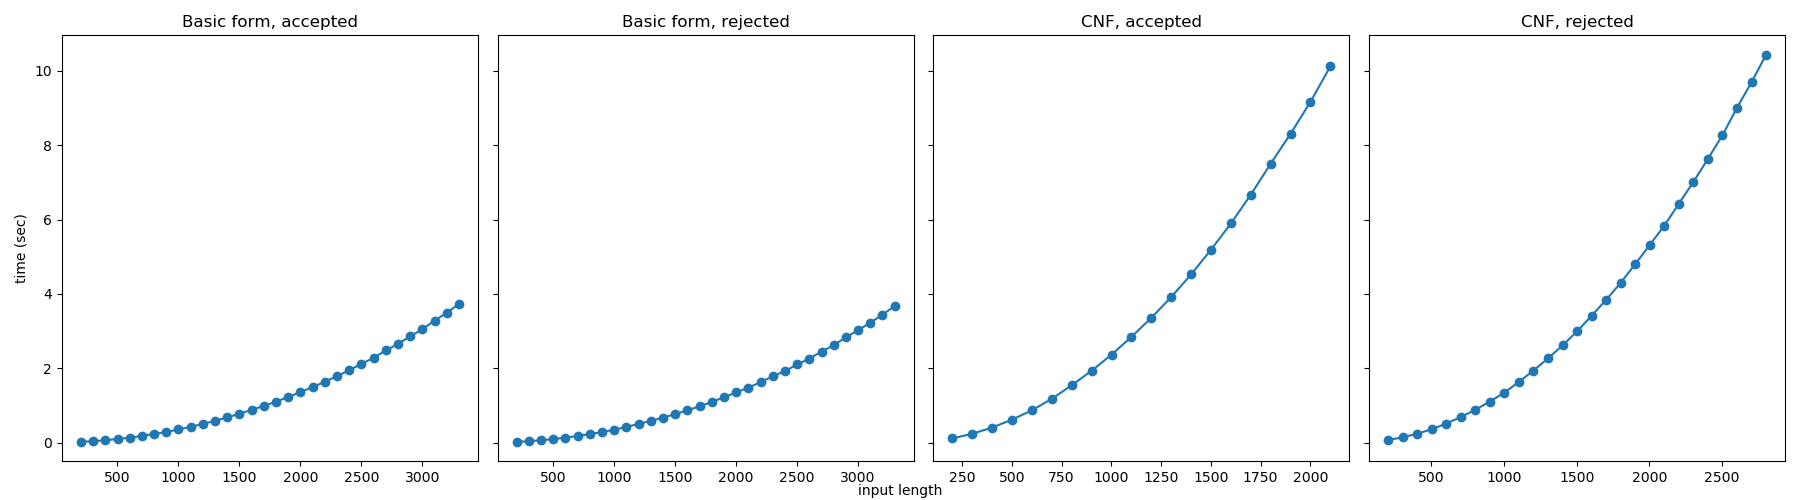
\includegraphics[scale=0.33]{compl_result_grammar_7.png}
  \caption{Grammar 7: $wcw^R$}
  \label{compl_result_grammar_7}
\end{figure}

\begin{figure}[h]
  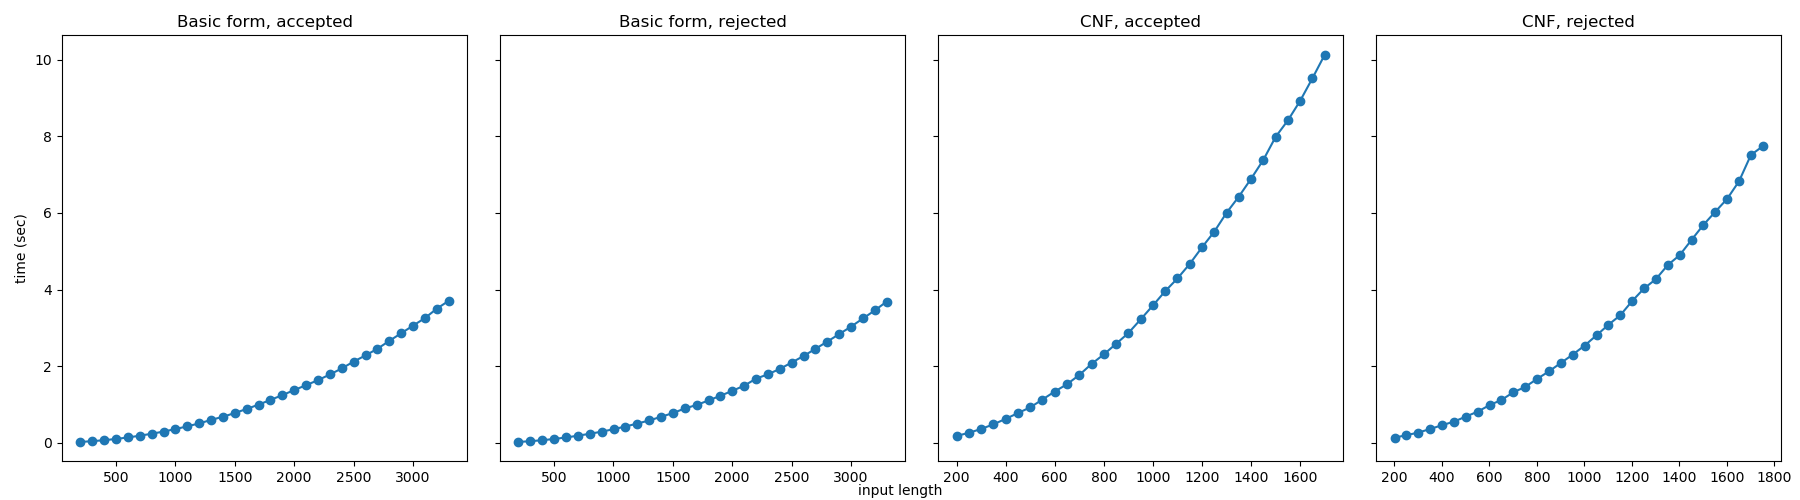
\includegraphics[scale=0.33]{compl_result_grammar_8.png}
  \caption{Grammar 8: $ww^R$}
  \label{compl_result_grammar_8}
\end{figure}

\begin{figure}[h]
  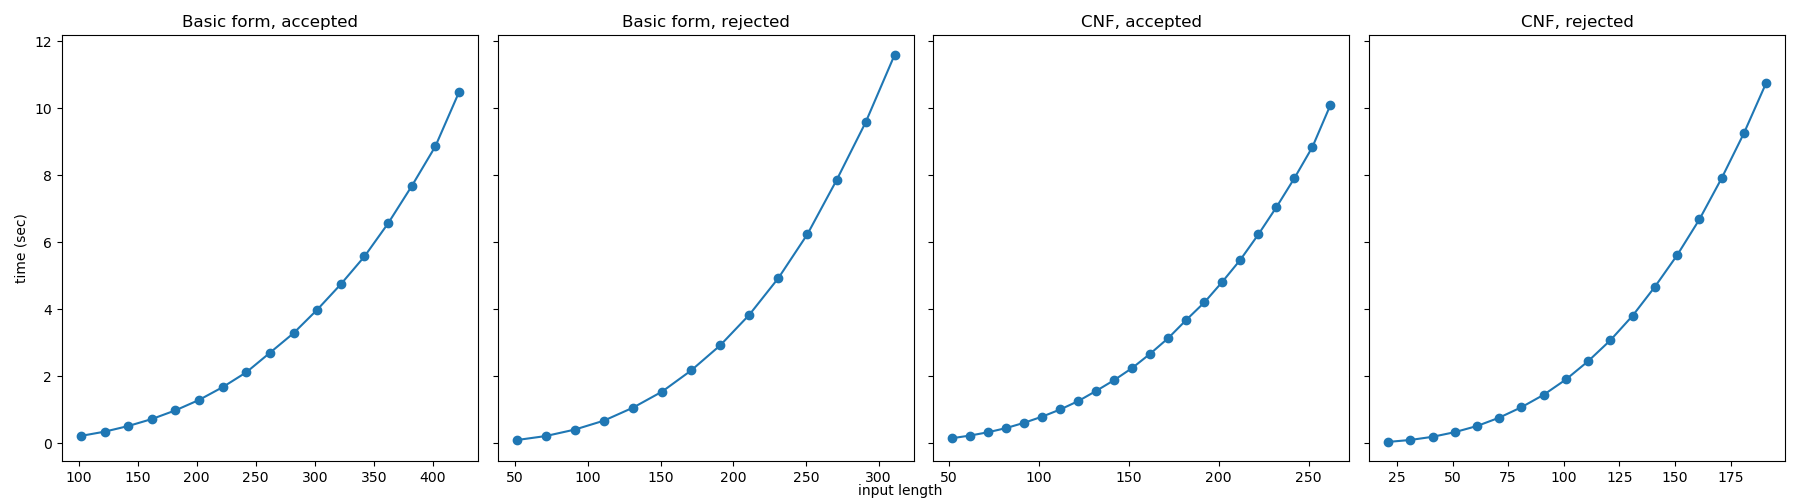
\includegraphics[scale=0.33]{compl_result_grammar_9.png}
  \caption{Grammar 9: $x2y: |x| \neq |y|$}
  \label{compl_result_grammar_9}
\end{figure}

\begin{figure}[h]
  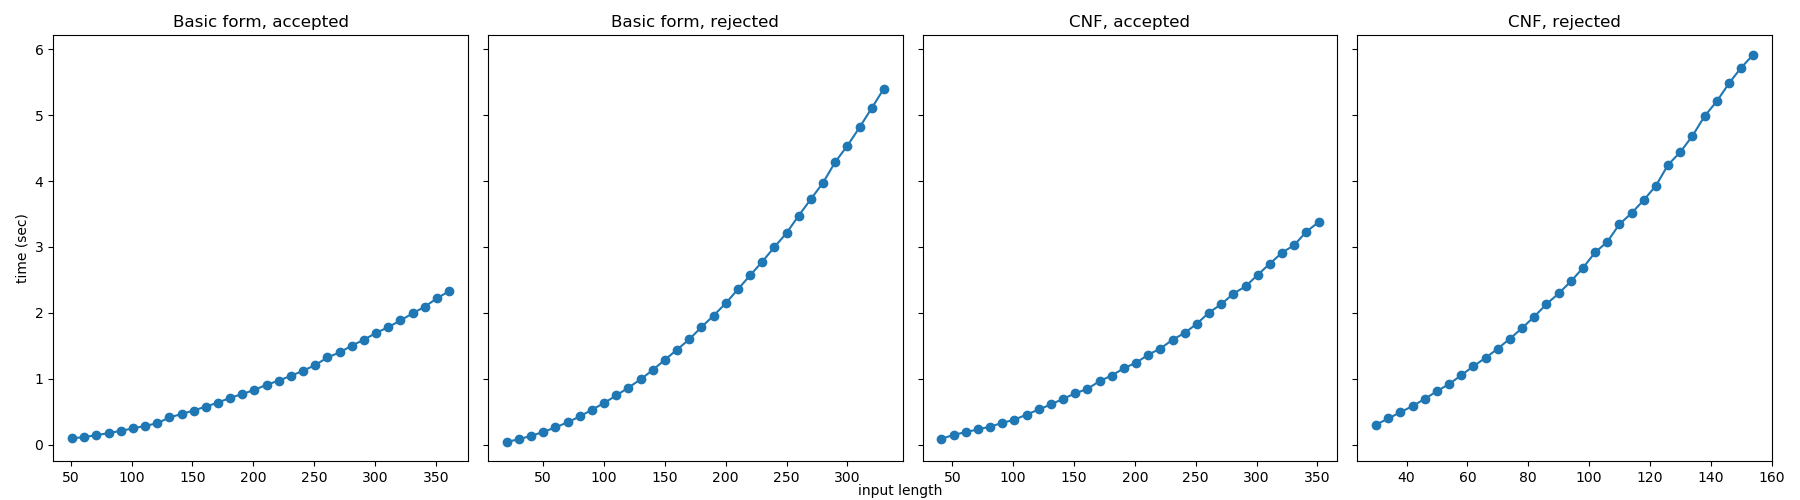
\includegraphics[scale=0.33]{compl_result_grammar_10.png}
  \caption{Grammar 10: regular expressions over 0 and 1}
  \label{compl_result_grammar_10}
\end{figure}

\begin{figure}[h]
  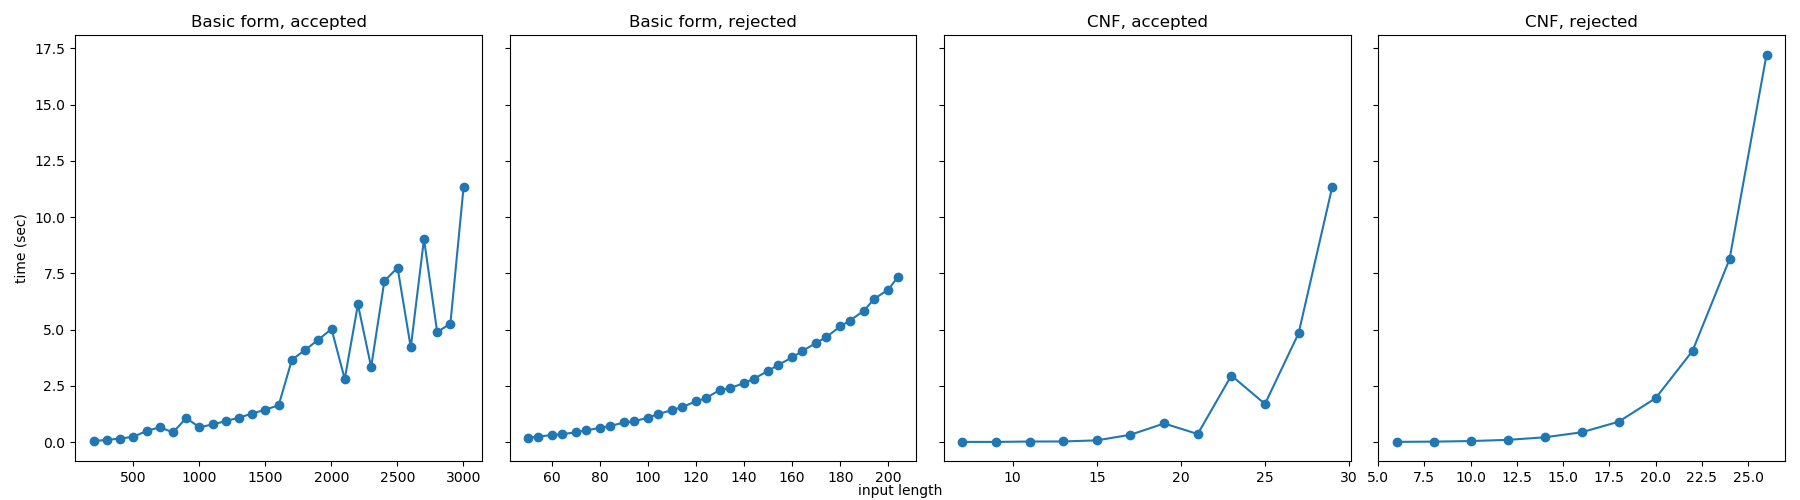
\includegraphics[scale=0.33]{compl_result_grammar_11.png}
  \caption{Grammar 11: $(ww)^C$}
  \label{compl_result_grammar_11}
\end{figure}

\begin{figure}[h]
  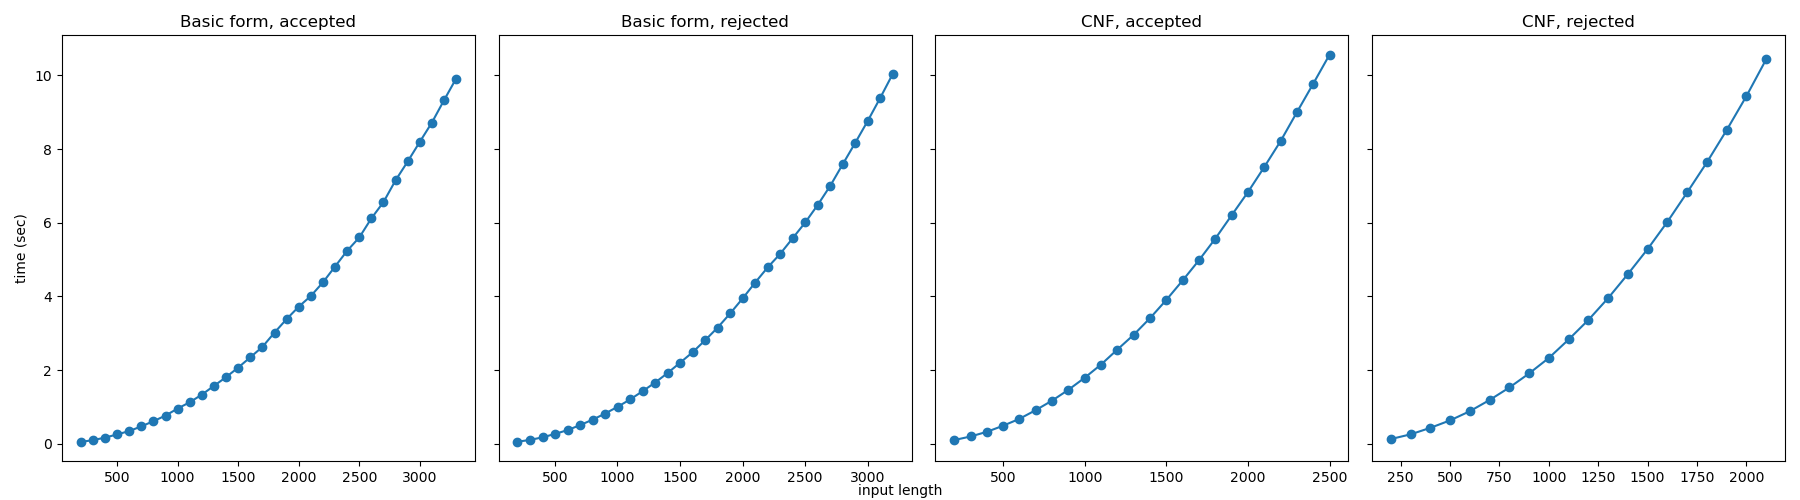
\includegraphics[scale=0.33]{compl_result_grammar_12.png}
  \caption{Grammar 12: $r^nd^nu^nr^n$}
  \label{compl_result_grammar_12}
\end{figure}

\begin{figure}[h]
  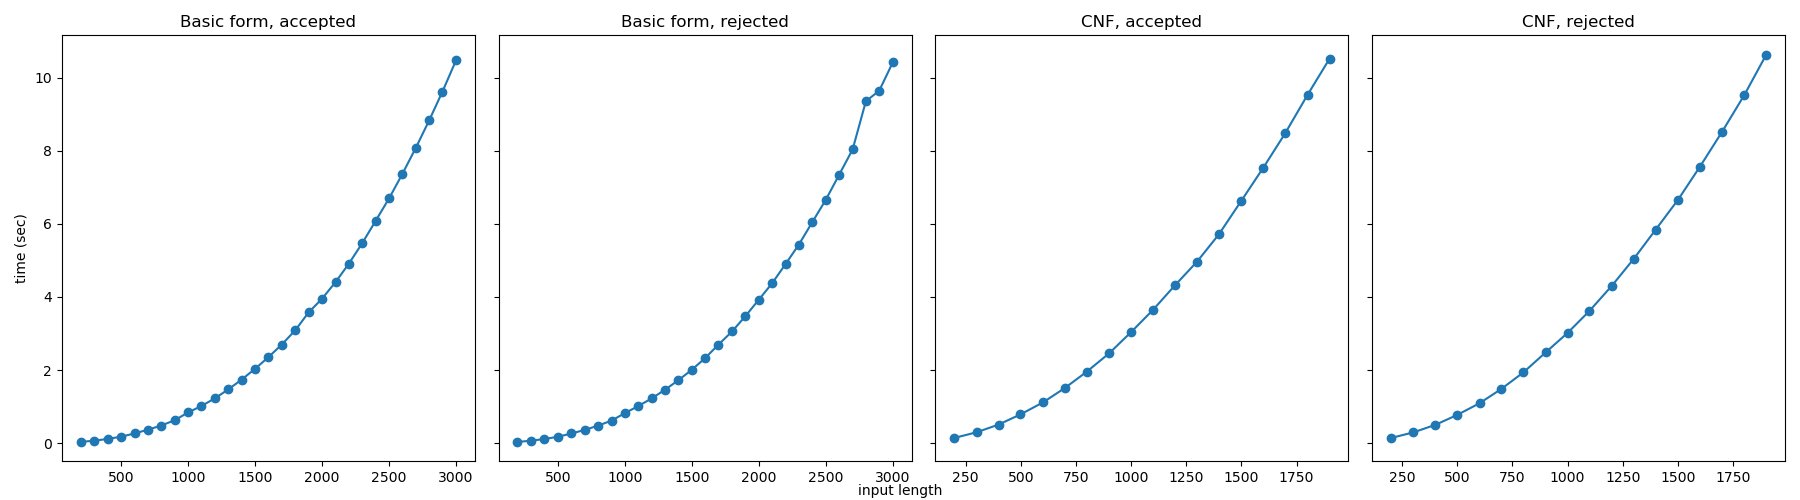
\includegraphics[scale=0.33]{compl_result_grammar_13.png}
  \caption{Grammar 13: $a^nc^nb^n$}
  \label{compl_result_grammar_13}
\end{figure}

\begin{figure}[h]
  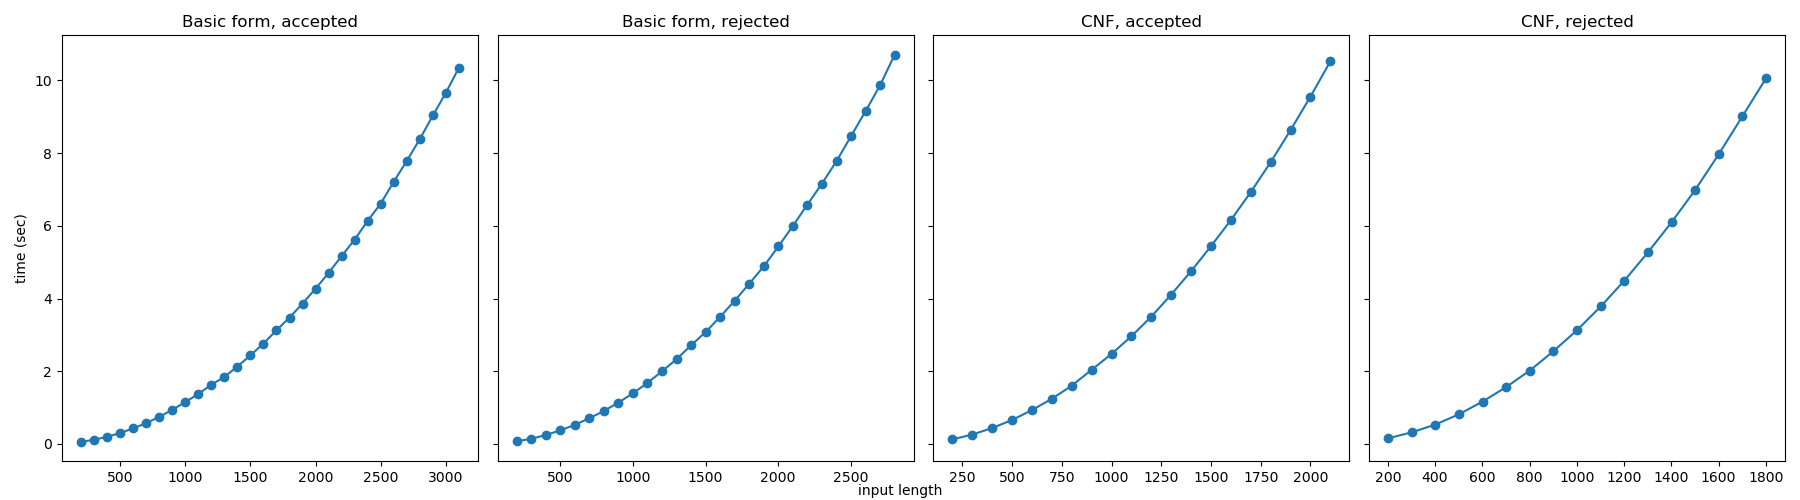
\includegraphics[scale=0.33]{compl_result_grammar_14.png}
  \caption{Grammar 14: $a^nb^mc^nd^m$}
  \label{compl_result_grammar_14}
\end{figure}

\begin{figure}[h]
  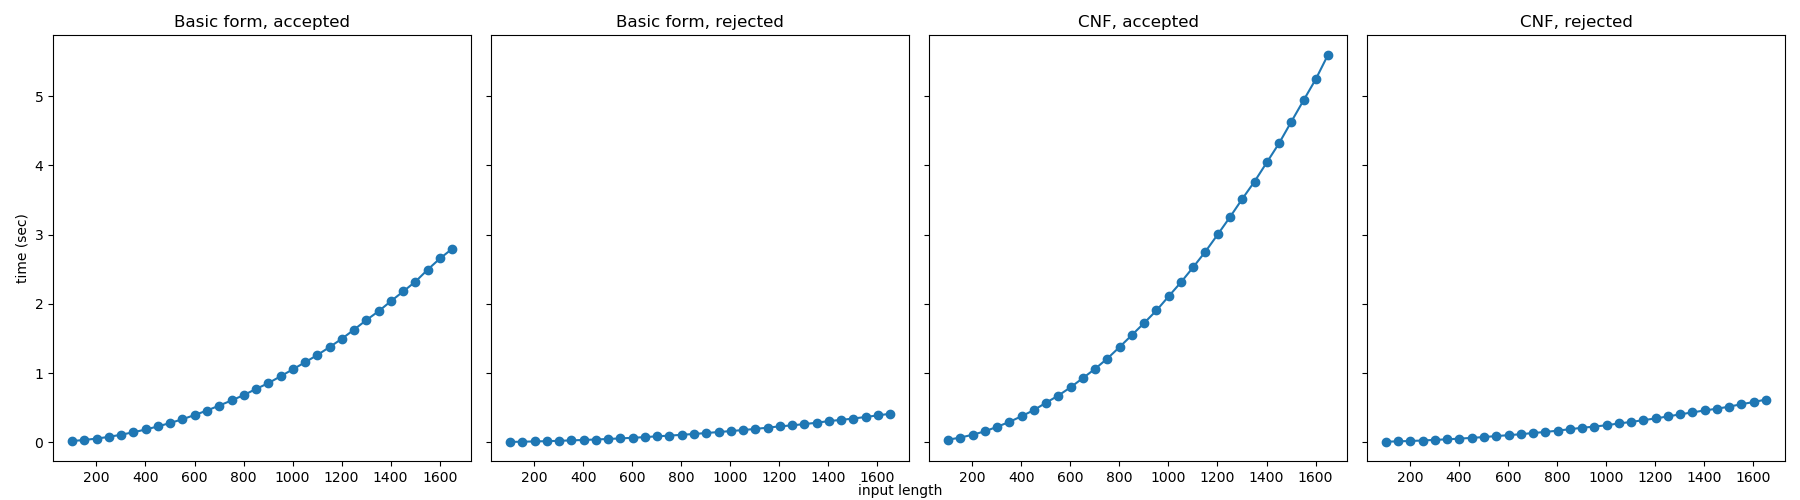
\includegraphics[scale=0.33]{compl_result_grammar_15.png}
  \caption{Grammar 15: $wcw$}
  \label{compl_result_grammar_15}
\end{figure}

\begin{figure}[h]
  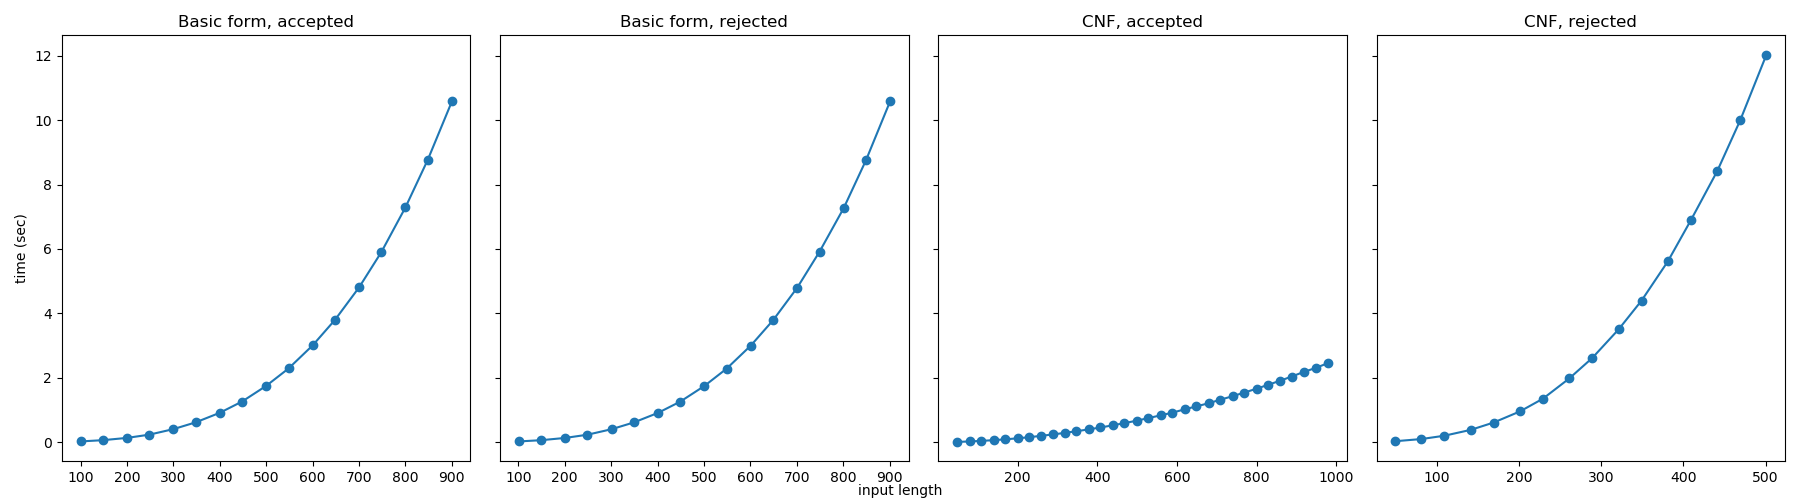
\includegraphics[scale=0.33]{compl_result_grammar_16.png}
  \caption{Grammar 16: $a^nb^ma^n$ where $2n \leq m \leq 3n$}
  \label{compl_result_grammar_16}
\end{figure}

\begin{figure}[h]
  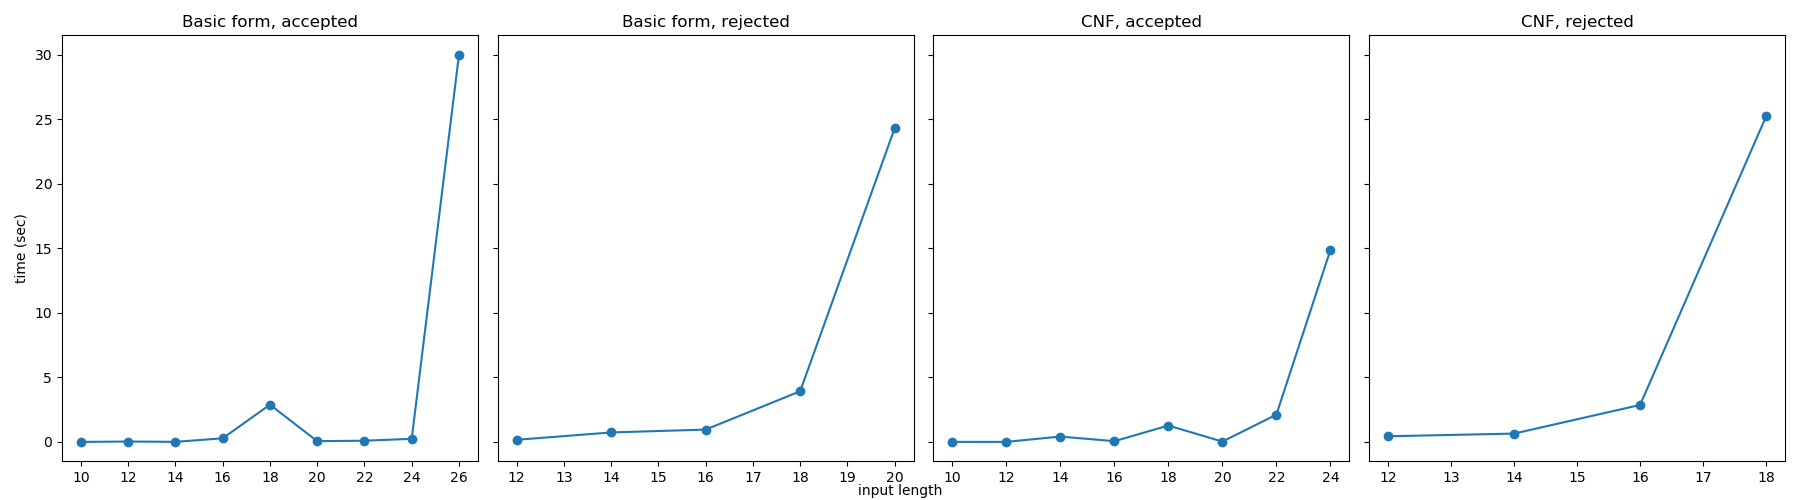
\includegraphics[scale=0.33]{compl_result_grammar_17.png}
  \caption{Grammar 17: $w: \#_a(w) = \#_b(w)$ and for prefix $v$ of $w: w: \#_a(w) \geq \#_b(w)$}
  \label{compl_result_grammar_17}
\end{figure}

\begin{figure}[h]
  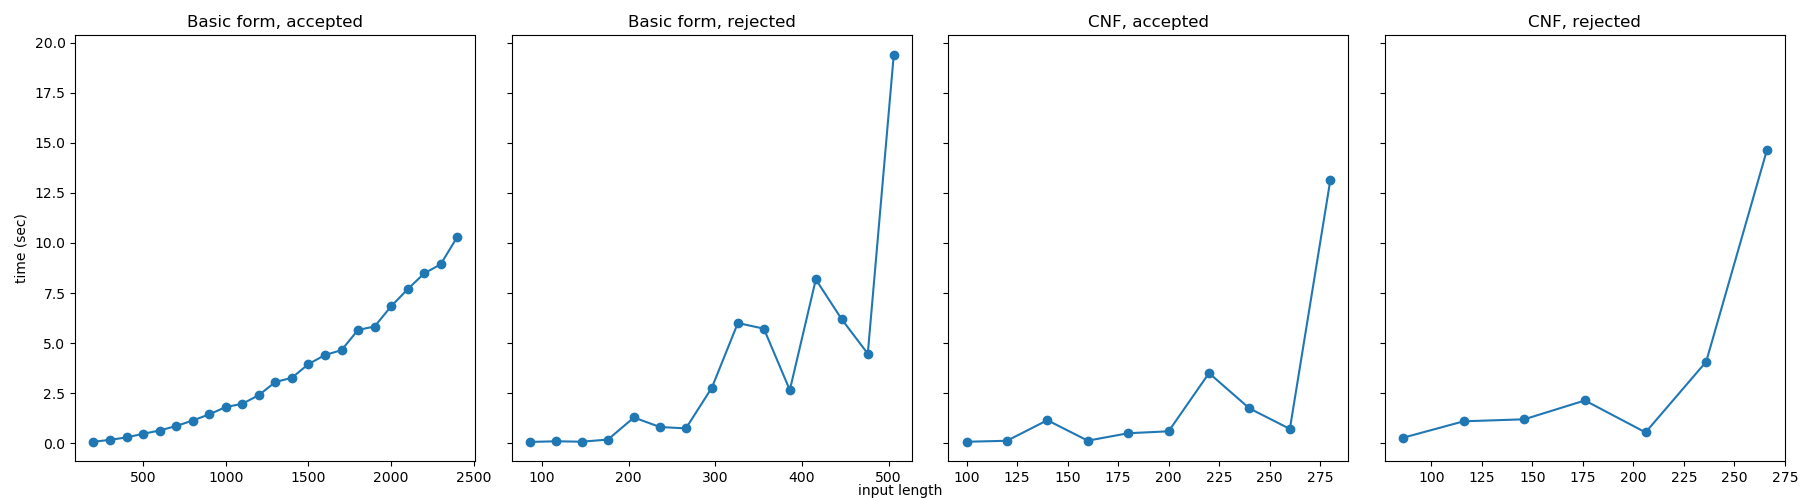
\includegraphics[scale=0.33]{compl_result_grammar_18.png}
  \caption{Grammar 18: $(l^nr^n)^k$ where $n$ does not increase for subsequent $k$s}
  \label{compl_result_grammar_18}
\end{figure}

\begin{figure}[h]
  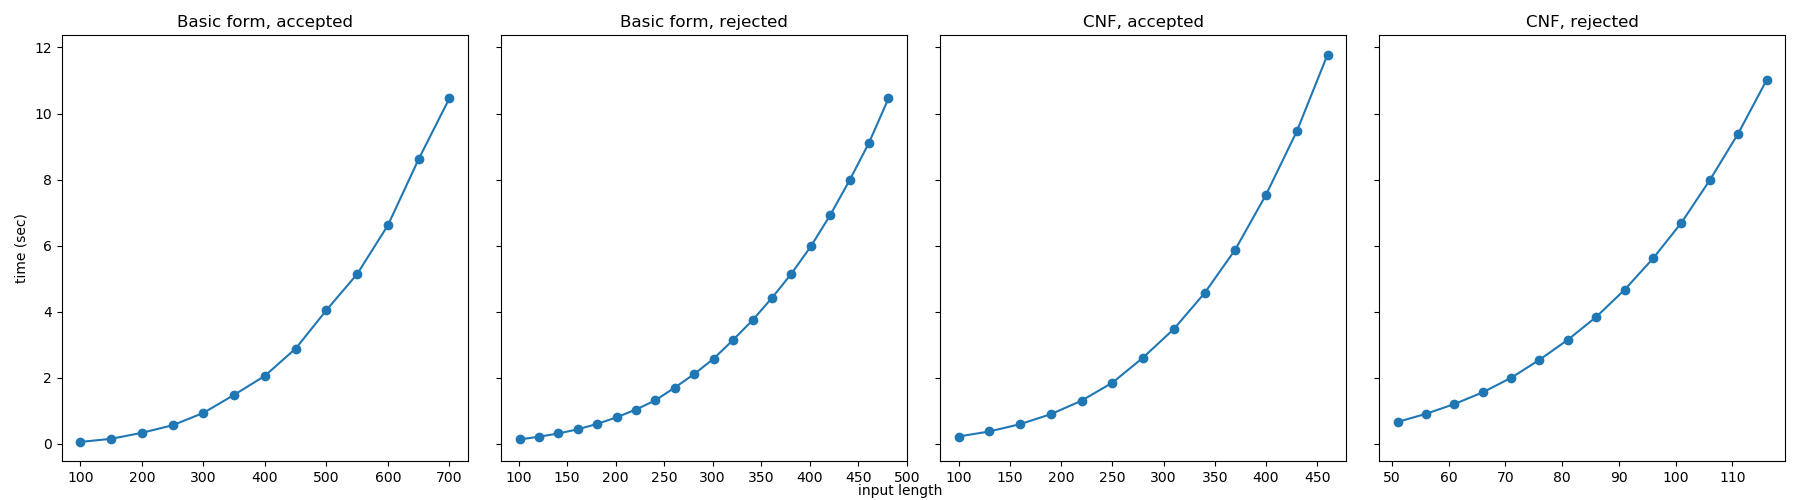
\includegraphics[scale=0.33]{compl_result_grammar_19.png}
  \caption{Grammar 19: $a^n c^m b^n$}
  \label{compl_result_grammar_19}
\end{figure}

\begin{figure}[h]
  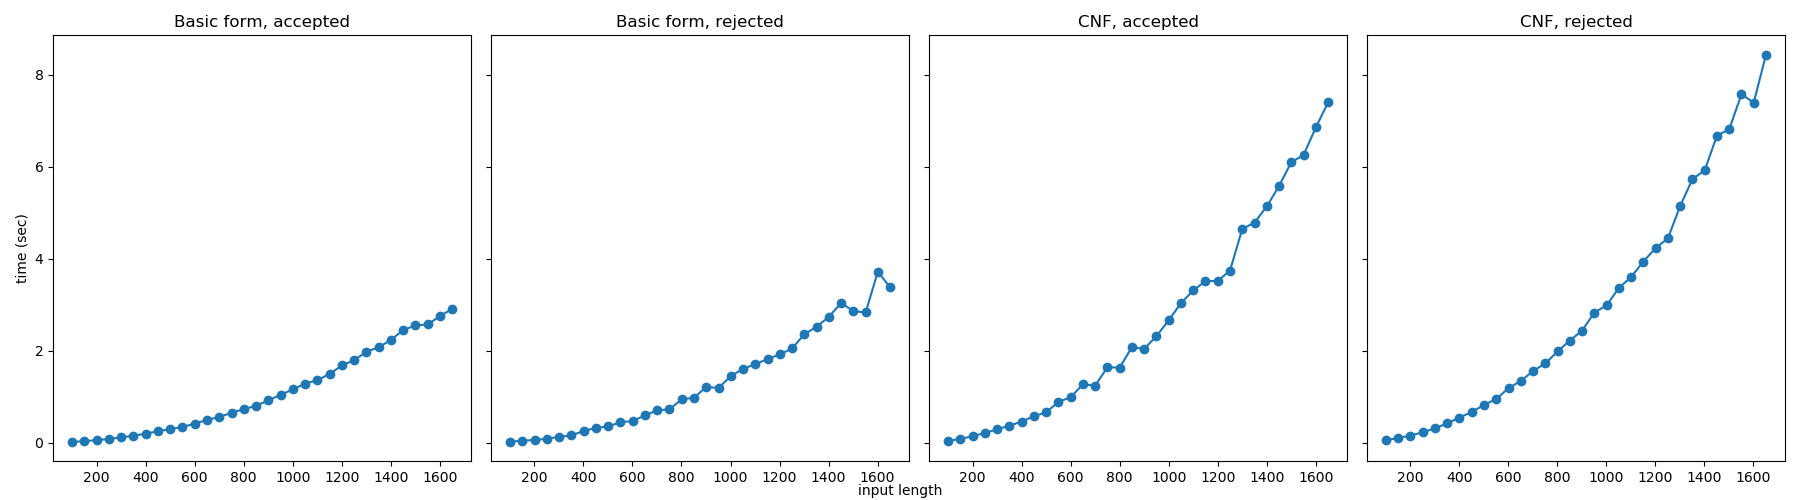
\includegraphics[scale=0.33]{compl_result_grammar_20.png}
  \caption{Grammar 20: $a^m b^n c^o d^p$ where $m+n = o+p$}
  \label{compl_result_grammar_20}
\end{figure}

These figures show that typically the tree search algorithm has a exponential growth but it starts to grow in quite high numbers. It it usually feasible to get the answer for inputs with lengths of hundres and often even thousands symbols.

Occasionally, thanks to the pruning heuristics the algorithm is able to tell practically immediately that there is no solution. This is the case of grammar 3 \ref{compl_result_grammar_3} and grammar 4 \ref{compl_result_grammar_4} in basic forms, making the complexity of this particular search constant. The grammar 3 has as the first rule, which it has to use to proceed further, $S \rightarrow A \wkpair{abc}{abc}$. If the input string does not end in $abc$ the regular expression check immediately detects that the input cannot be matched, prunes the only branch and the search is finished.

Similarly in the case of grammar 4, any inputs that are longer than seven symbols need to end with symbol $a$ and can be reached only by using $S \rightarrow Q \wkpair{a}{a}$ as the first rule. The regular expression check immediately prunes this branch. The rest of the tree is searched very quicky, because the only other possible starting rule is $S \rightarrow A B C D E F G$, there are not many states that can be reached from it, so this part of the tree is always small.

After conversion of the grammar to CNF, the complexity usually goes up. This is because the transformation adds a lot more rules and thus the state space expands more rapidly, there is also longer paths from the starting non-terminal to the final string (containing only terminals) making the tree deepr. Also, the node precedence heuristics and the pruning have harder time, because many rules contain non-terminals only and most of the heuristics work with terminals. The most extrem case is the grammar 3 where the tree search is very effective for grammar in basic form (as discussed, in case of rejecting inputs the result is immediate), but has very bad effectivness for in CNF. The maximum length of input it can answer within 10 second is about 13--14 symbols.

The worst results for grammar in the basic form are in the case of grammar 17 \ref{compl_result_grammar_17}. For all other grammars, the input length can be in hundrets and in most cases more that a thousand and more. With grammar 17 the tree search can handle only inputs with length of about 25 symbols within 10 seconds.

\section{Comparing different inputs of the same length}
Aa for grammars 1-4 the only unusual inputs that are possible are inputs with a unexpected termianal, a terminal which is not in the set of the grammar terminals.
In case of grammar 5 it the key input part is the $ctg$ it can be at the beginning, or in the middle or at the end.

\section{Testing the efficiency of WK-CYK}

I have tested the WK-CYK algorithm in a similar manner as the tree search. This time not all grammars can be used due to limitations of WK-CYK. Grammars must be in CNF form and grammars 5, 19 and 20 cannot be used at all, since WK-CYK requires the complementarity relation to be identity, which is not the case of these three grammas. Therefore there are 17 grammars that can be tested. The script \textit{wk\_cyk\_test} runs two tests for each of these grammrs. One with inputs that should be accepted and one with inputs that should be rejected. Again, each test increases the input string length until it the computation lasts more that a limit of 10 seconds. The output of each test is again a table similar to \ref{tab:wk_cyk_res}. The entire output can be remade by running the script again and is attached in file \textit{ouput/wk\_test.txt}.

\begin{figure}[h]
\centering
  \caption{An output of the WK-CYK time complexity test}
  \label{tab:input_compl_test}
\begin{tabular}{ |l|l|l|  }
  \hline
  \multicolumn{3}{|l|}{Test 1} \\
  \hline
  Grammar & \multicolumn{2}{|l|}{$a(aa)^*$} \\
  Rules / NTs / Ts & \multicolumn{2}{|l|}{2/1/1} \\
  Should accept & \multicolumn{2}{|l|}{Yes} \\
  Timeout & \multicolumn{2}{|l|}{7 seconds} \\
  \hline
  Input length & Time & Accepted \\
  \hline
  3 & 0.0 & TRUE \\
  5 & 0.0 & TRUE \\
  7 & 0.0 & TRUE \\
  9 & 0.01 & TRUE \\
  11 & 0.03 &  TRUE \\
  13 & 0.07 &  TRUE \\
  15 & 0.15 &  TRUE \\
  17 & 0.29 &  TRUE \\
  19 & 0.53 &  TRUE \\
  21 & 0.88 &  TRUE \\
  23 & 1.45 &  TRUE \\
  25 & 2.31 &  TRUE \\
  27 & 3.49 &  TRUE \\
  29 & 5.23 & TRUE \\
  31 & 7.55 & TRUE \\
  33 & 10.67 & TRUE \\

  \hline
\end{tabular}
\end{figure}

It turns out that the WK-CYK gives very similar performance in all tests --- for all the grammars and regardless whether the input is accepted or not. The figure \ref{fig:wk_cyk_grammar1} to the right shows a result for the first test which is very similar to all the others.

These results comfirm the claim made by authors of WK-CYK, that the complexity with regards to the input length is $O(n^6)$. The figure \ref{fig:wk_cyk_grammar1} shows the same test with the input lengths raised to the power of six, which can be considered to be a number of operations. The curve is then very close to linear.

When the results of the WK-CYK and state space search are compared, the advantage of state space search is the actual speed in most cases. The results in the previous sections showed that of all the grammars only one (grammar 17) was slower in the basic form when analysed by tree search, then when analysed by WK-CYK. After transformation to CNF two more grammars (grammar 3 and 11) were comparable or slower when analysed by tree search.

Another advantage of state space search is the flexibility regarding the grammar. It does not require to work with grammar in CNF. Also, it does not require the complementarity relation to be identity. Even though it is always possible to transform any WK grammar to the WK-CNF and it is always possible to further transform the grammar to use only the identity as the relation, this can significantly add to the grammar complexity.

The advantage of WK-CYK, on the other hand, is its universality. It has roughly the same speed every time, it does not significantly depend on the grammar (increasing number of rules adds a liitle bit) and it does not matter, if the input is going to be accepted or not. For very complicated grammars, especially with lots of rules or long derivations from the starting symbol to the final string, WK-CYK still might be more practical.

\begin{figure}[h]
  \centering
  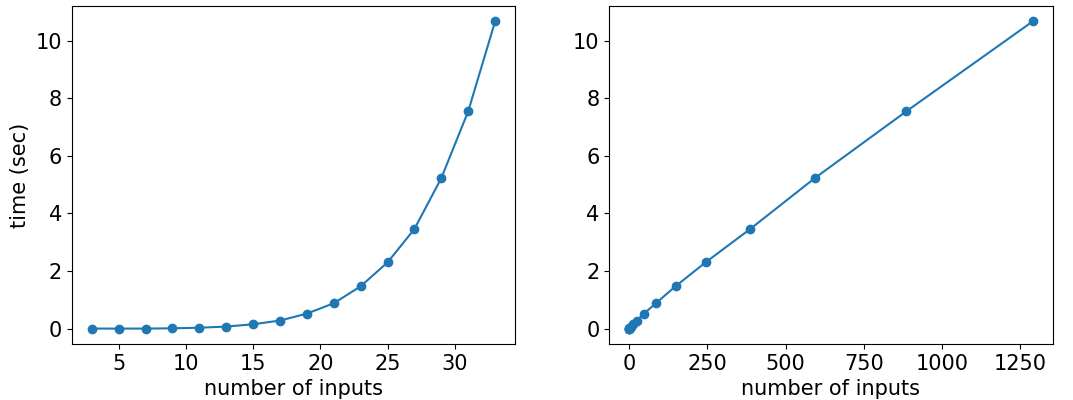
\includegraphics[scale=0.5]{wk_cyk_test_1.png}
  \caption{WK-CYK test result}
  \label{fig:wk_cyk_test1}
\end{figure}

The limit of ten seconds is reached by WK-CYK when the input has about 33 symbols.

\chapter{Conclusion}
Future work: It is possible to implement other pruning algorithms and test if they contribute to speed. It is possible to use the case where the algorithm was the least effective to try to desing new, better (generally or specificcaly for that case) node precedence heuristics.
Implement paralelism.
